% Vorlage: https://www.pfsr.de/latex

% -- Anfang Präambel
\documentclass[german,  % Standardmäßig deutsche Eigenarten, englisch -> english
parskip=full,  % Absätze durch Leerzeile trennen
%bibliography=totoc,  % Literatur im Inhaltsverzeichnis (ist unüblich)
%draft,  % TODO: Entwurfsmodus -> entfernen für endgültige Version
]{scrartcl}

\usepackage[utf8]{inputenc}  % Kodierung der Datei
\usepackage[T1]{fontenc}  % Vollen Umfang der Schriftzeichen
\usepackage[ngerman]{babel}  % Sprache auf Deutsch (neue Rechtschreibung)

% Mathematik und Größen
\usepackage{amsmath}
\usepackage{amsfonts}
\usepackage[locale=DE,  % deutsche Eigenarten, englisch -> US
separate-uncertainty,  % Unsicherheiten seperat angeben (mit ±)
]{siunitx}
\usepackage{physics}  % Erstellung von Gleichungen vereinfachen

\usepackage{graphicx}  % Bilder einbinden \includegraphics{Pfad/zur/Datei(ohne Dateiendung)}

% Gestaltung
\usepackage{booktabs}  % schönere Tabellen
\usepackage[toc]{multitoc}  % mehrspaltiges Inhaltsverzeichnis
\usepackage{csquotes}  % Anführungszeichen mit \enquote
\usepackage{caption}  % Anpassung der Bildunterschriften, Tabellenüberschriften
\usepackage{subcaption}  % Unterabbildungen, Untertabellen, …
\usepackage{enumitem}  % Listen anpassen
\setlist{itemsep=-10pt}  % Abstände zwischen Listenpunkten verringern

% Manipulation des Seitenstils
\usepackage[headtopline = .5pt]{scrlayer-scrpage}

% Bibliographie
\usepackage[backend=biber]{biblatex}
\addbibresource{bibliography.bib}

% SI-Einheiten darstellen
\usepackage{siunitx}

% Tabellen mit geteilten Zeilen
\usepackage{multirow}

% Kopf-/Fußzeilen setzen
\pagestyle{scrheadings}  % Stil für die Seite setzen
\clearmainofpairofpagestyles  % Stil zurücksetzen, um ihn neu zu definieren
\automark{section}  % Abschnittsnamen als Seitenbeschriftung verwenden
\ofoot{\pagemark}  % Seitenzahl außen in Fußzeile
\ihead{\headmark}  % Seitenbeschriftung mittig in Kopfzeile

\usepackage[hidelinks]{hyperref}  % Links und weitere PDF-Features

% TODO: Titel und Autor, … festlegen

%\newcommand\norm[1]{\left\lVert#1\right\rVert} % Norm

\newcommand*{\titel}{Beschleunigermas­senspektrometrie und Methoden zur Altersbestimmung}
\newcommand*{\autor}{Sebastian Thiede, Alexander Lettau}
\newcommand*{\abk}{BM}
\newcommand*{\betreuer}{Dr. Johannes Lachner, Dr. Georg Rugel}
\newcommand*{\messung}{16.12.2021}
\newcommand*{\ort}{Helmholtz-Zentrum Dresden Rossendorf, DREAMS}

\hypersetup{pdfauthor={\autor}, pdftitle={\titel}}  % PDF-Metadaten setzen

% automatischen Titel konfigurieren
\titlehead{Praktikum des IKTP \abk \hfill TU Dresden}
\subject{Versuchsprotokoll}
\title{\titel}
\author{\autor}
\date{\begin{tabular}{ll}
Protokoll: & \today\\
Messung: & \messung\\
Ort: & \ort\\
Betreuer: & \betreuer\end{tabular}}

% -- Ende Präambel

\begin{document}
\begin{titlepage}
\maketitle  % Titel setzen
\tableofcontents  % Inhaltsverzeichnis setzen
\end{titlepage}

% ----- DOKUMENT ANFANG -----

\section{Aufgabenstellung}
Die Beschleunigermas­senspektrometrie (AMS) ist ein wichtiges Werkzeug zur Trennung und Detektierung von Nukliden.
Eine der häufigsten Anwendungen ist die Altersbestimmung von Proben aus der Natur durch Messung der Konzentration verschiedener Nuklide, die auf der Erdoberfläche durch kosmische Strahlung entstehen.
Im Gegensatz zu anderen Verfahren der Massenspektrometrie erreicht man bei der AMS eine sehr gute Unterdrückung atomarer und molekularer Isobare.
Die Messzeiten sind relativ kurz und es lassen sich auch kleine Proben untersuchen.

In diesem Versuch wurde der Beschleuniger DREAMS (DREsden AMS) vorgestellt.
Die generelle Handhabung wurde anhand folgender praktischer Aufgaben kennengelernt:
\begin{itemize}
  \item Inbetriebnahme eine Sputter-Ionenquelle und Erzeugung negativer Ionen
  \item Strahlentransport eines Isotopenpaares durch den Beschleuniger
  \item Kalibrierung der Verstärkung der gasgefüllten Ionistationskammer
  \item Aufnahme von Messwerten in der gasgefüllten Ionisationskammer
\end{itemize}

Zur Auswertung sind folgende Aufgaben zu bearbeiten:
\begin{itemize}
  \item Berechnung der Teilchenenergien nach dem Beschleuniger
  \item Plotten des Stromes des Ionenstrahls im Faraday Cup
  \item Abschätzung des Energieverlustes des Ionenstrahls in einer dünnen Folie
  \item Abschätzung des Energieverlustes des Ionenstrahls in Isobutan (Gas in der Ionisationskammer)
  \item Plotten der gemessenen Spektren und Identifikation der Ionen
  \item Berechnung der Konzentration von Radionukliden in einer unbekannten Probe
\end{itemize}

\section{Theorie}

\subsection{organische Szintillatoren}

Szintillatoren sind  Materialien die bei bestrahlung mit energiereichen Photonen oder geladenen Teilchen angeregt werden und die Anregungsenergie in Form von Licht wieder abgeben. Organische Szintillatoren bestehen wie der Name schon vermuten lässt vorwiegend aus Kohlenstoff, Wasserstoff, Sauerstoff und Stickstoff wie es auch in z.B. menschlichem Gewebe der Fall ist. Es liegt daher nahe Detektoren auf Basis organischer Szintillatoren für die Dosismessung im Strahlenschutz zu verwenden. Organische Szintillatoren bestehen typischerweise aus zwei Komponenten: Einem primären Fluoreszenzstoff (z.B. auf Basis von Polyvinyltoluol) und einem \glqq Wellenlängenschieber \grqq{} (z.B. POPOP) da die vom primären Fluoreszenzstoff abgegebenen UV-Strahlen in den meisten durchsichtigen Materialien eine nur sehr geringe Reichweite besitzen.

\subsection{Wechselwirkung von Photonen mit Materie}

Obwohl Photonen in vieler Weise mit Materie wechselwirken können sind für diesen Versuch nur zwei Prozesse von wesentlicher Bedeutung: Die Compton-Streuung und der Photoeffekt. In den folgenden Abschnitten werden beide näher erläutert.

\subsubsection{Photoeffekt}

Der Photoeffekt beschreibt die Anregung von Elektronen durch Absorption eines Photons.
Für den HPGe-Detektor ist vor allem der innere photoelektrische Effekt von Bedeutung. Er beschreibt die Zunahme der Leitfähigkeit eines Halbleiters durch Bildung von nicht aneinander gebundenen Elektron-Loch-Paaren. Der HPGe-Detektor besteht aus einem hochreinen Germanium-Kristall der zwischen einem $n^{+}$ Kontakt (typ. durch Lithium-eindiffusion) am positiven Spannungspol und einem $p^{+}$ Kontakt (typ. durch Bor-implantation) am negativen Spannungspol sitzt; Der Detektor insgesamt entspricht einer Halbleiterdiode in Sperrichtung. Trifft ein Photon auf den Detektor und erzeugt ein Elektron-Loch-Paar werden durch die anliegende Spannung Elektron und Loch abgesaugt und bilden so einen detektierbaren Verschiebungsstrom. Dafür muss das einfallende Photon natürlich genügend Energie besitzen um die Bandlücke zu überwinden (Für Germanium \SI{0.67}{\electronvolt}), praktisch jedoch deutlich mehr um das Siganl-Rausch-Verhältnis groß genug zu bekommen. So werden bei einfallenden Photonen von \SI{1}{\mega\electronvolt} etwa \num{3e5} Elektron-Loch-Paare erzeugt \cite{HPGe-Detektor}. Da bei Raumtemperatur eine ständige thermische Anregung der Elektronen enormes Signalrauschen verursachen würde ist eine Abkühlung mit flüssigem Stickstoff notwendig.
Für den zu kalibrierenden Detektor ist vor allem der äußere photoelektrische Effekt von Bedeutung, genauer für den Photoelektronenvervielfacher (Abb. \ref{theorie_PEV}).

\begin{figure}[ht]
	\centering
  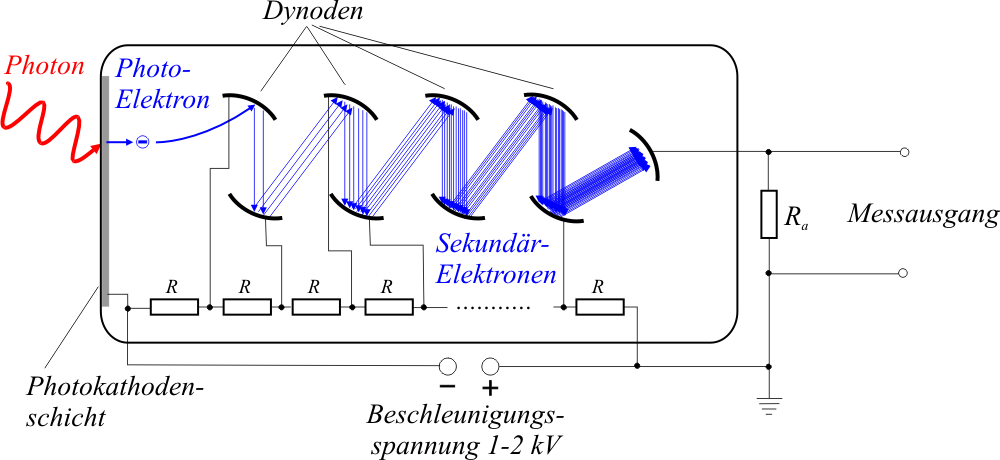
\includegraphics[width=0.85\textwidth]{images/Photomultiplier_schema_de.png}
	\caption{Schematik Photoelektronenvervielfacher}
	\label{theorie_PEV}
\end{figure}

Dort werden durch das Szintillationsphoton Elektronen aus einer Photokathode ausgeschlagen, durch angelegte Spannung zur ersten Dynode beschleunigt wo sie mit der gewonnenen kinetischen Energie weitere Elektronen auschlagen. Dieser Prozess wird einige male wiederholt bis ein messbarer elektrischer Impuls an der Anode entstehen kann.

\subsubsection{Compton-Streuung}

\subsection{Weitwinkel-Compton-Koinzidenz-Methode}

\section{Versuchsaufbau}
Eine Schematische Zeichnung der DREAMS-Anlage ist in Abb. \ref{Auswertung_Bild_DREAMS} zu finden.
\begin{figure}[ht]
	\centering
    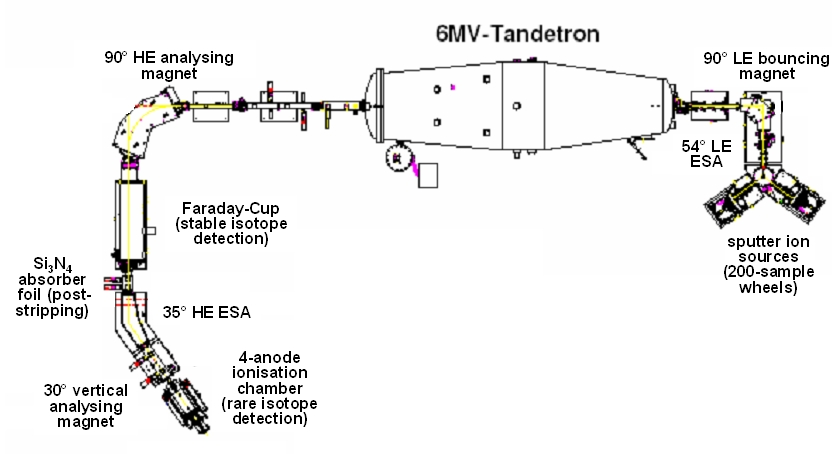
\includegraphics[width=0.85\textwidth]{Pictures/DREAMS.png}
	\caption{Schematik DREAMS \cite{Bild_DREAMS}}
	\label{Auswertung_Bild_DREAMS}
\end{figure}
Sie besteht aus folgenden Komponenten:
\begin{itemize}
    \item Sputter-Ionenquelle
    \item \ang{54} elektrostatischer Analysierer auf der Niederenergieseite
    \item \ang{90} Ablenkmagnet auf der Niederenergieseite
    \item \SI{6}{\mega\electronvolt} Tandem-Beschleuniger
    \item \ang{90} Ablenkmagnet auf der Hochenergieseite
    \item Faraday-Cups zur detektierung stabiler Isotope
    \item SiN Absorberfolie
    \item \ang{35} elektrostatischer Analysierer auf der Hochenergieseite
    \item \ang{30} vertikaler Analysemagnet
    \item Ionisationskammer mit 4 Anoden
\end{itemize} % weitere erklärungen?

\section{Experimenteller Teil}
Im ersten Teil der Auswertung verfolgen wir im Wesentlichen Ionen durch die Anlage.
Untersucht werden soll dabei eine vorbereitete BeO-Probe, genannt \glqq 153BeO\grqq{}, und die Proben \glqq 13KY\grqq{}, \glqq 14KY\grqq{}, \glqq 16KY\grqq{} und \glqq 17KY\grqq{}.
Im zweiten Teil betrachten wir aufgenommene Spektren und untersuchen eine unbekannte Probe.

\subsection{Auf dem Weg zum Beschleuniger}
Nach der Produktion der negativen Ionen durch sputtern werden diese wie erwähnt mit insgesamt \SI{29}{\kilo\electronvolt} beschleunigt.
Sie durchlaufen dann einen elektrostatischen Analysierer und einen ersten Ablenkmagneten.
Das Ziel hier ist eine Ionenmasse vorzuselektieren.
Da wir BeO untersuchen sind mögliche gesuchte Ionen $^{9}\text{Be}^{16}\text{O}^{-}$ (stabiles Beryllium-Iosotop) und $^{10}\text{Be}^{16}\text{O}^{-}$ (radioaktives Beryllium-Iostop mit einer Halbwertszeit von \num{1.387e6} Jahren).
Zu beachten ist, dass Sauerstoff zwar zum Großteil aus $^{16}$O besteht, jedoch in geringen Mengen auch die stabilen Isotope $^{17}$O und $^{18}$O vorkommen können, was eine gewisse Quelle für Unsicherheiten ist.
Wir kennen die kinetische Energie $E_{\text{kin}}$, den Ladungszustand $q_{\text{ion}}$, die Masse der Ionen $m_{\text{ion}}$ und den Krümmungsradius der weiterführenden Trajektorie $\rho$.
Daher kann man durch geeignete Wahl der Stärke des Magnetfeldes die Ionenmasse auswählen:
\begin{gather}
    B \rho = \frac{p_{\text{ion}}}{q_{\text{ion}}} = \frac{\sqrt{2m_{\text{ion}}E_{\text{kin}}}}{q_{\text{ion}}}
    \label{Auswertung_eq_Magnet}
\end{gather}
Ionen mit einer anderen Masse oder anderem Ladungszustand haben im Magneten eine anders gekrümmte Trajektorie und gelangen daher nicht durch die Eintrittsöffnung zum Beschleuniger.
Negative Ionen mit einem anderen Ladungszustand als 1 treten jedoch nur sehr selten auf.
(Tatsächlich lässt sich wie in Gleichung \ref{Auswertung_eq_Magnet} zu sehen nur nach $\frac{\sqrt{m_{\text{ion}}}}{q_{\text{ion}}}$ selektieren.
Ionen mit vierfacher Masse und doppelter Ladung würden also auch weiterkommen. Derart schwere Teilchen sind jedoch fast gar nicht in der Probe vorhanden.)
An dieser Stelle lässt sich jedoch nicht unterscheiden zwischen Molekularen isobaren, so zum Beispiel zwischen $^{10}\text{Be}^{16}\text{O}^{-}$ und $^{9}\text{Be}^{17}\text{O}^{-}$ (wobei $^{17}\text{O}$ in der Natur sehr selten vorkommt) oder $^{10}\text{Be}^{16}\text{O}^{-}$ und $^{10}\text{B}^{16}\text{O}^{-}$ ($^{10}\text{B}$ entsteht beim Beta-Zerfall von $^{10}\text{Be}$).
Ebenfalls wichtig ist, dass hier keine leichten Moleküle oder Ionen mit einem anderen Ladungszustand als 1 vorkommen, theoretisch vorhandene schwere Moleküle könnten jedoch hier mit höheren Ladungszuständen auftauchen.
Für $\rho$ war ein Wert von \SI{0.4}{\metre} gegeben.
Damit ergeben sich für einfach negativ geladene Ionen folgende benötigte Magnetfeldstärken:
\begin{table}[H]
  \centering
  \caption{Benötigte Magnetfeldstärken im ersten Ablenkmagneten für Ionen vor dem Beschleuniger}
  \begin{tabular}{|c|c|}
    \hline
    Ion & Magnetfeldstärke / \si{\tesla} \\
    \hline
    $^{9}\text{Be}^{16}\text{O}^{-}$ & \num{-0.306} \\
    \hline
    $^{10}\text{Be}^{16}\text{O}^{-}$ & \num{-0.313} \\
    \hline
  \end{tabular}
  \label{Auswertung_tab_Ionenenergien_vor_Besch}
\end{table}
Um diese Magnetfelder anzulegen ist im besten Fall eine Kalibrierung des Magneten vorhanden, die jedoch in diesem Versuch nicht durchgeführt wurde.
Stattdessen haben wir die chemisch reine Probe 153BeO genutzt, um die Stromstärke zu bestimmen, welche der Magnetfeldstärke zur Selektion von BeO$^{1-}$ entspricht.
Diese kann dann als Vergleichswert dienen, um aus den Verhältnissen der Magnetfeldstärken bzw. Stromstärken die Teilchen zu identifizeren.
Dieses Verhältnis folgt aus Formel \ref{Auswertung_eq_Magnet}: $\frac{B_1}{B_2} = \sqrt{\frac{m_1}{m_2}}$.
Vor dem Tandem ergibt sich die Energie der BeO$^{1-}$ Teilchen zu $E = q \cdot U_{\text{Ionenquelle}}$.
Nach Formel \ref{Auswertung_eq_Magnet}, mit dem Radius des Magneten $\rho = \SI{0.4}{\metre}$, ergibt sich für das zugehörige Magnetfeld $B = \SI{0.306}{\tesla}$.
Messungen am Magneten ergaben eine zugehörige Stromstärke von $I = \SI{61.05}{\ampere}$.
Die Masse eines unbekannten Teilchens ergibt sich damit zu:
\begin{equation}
    m_2 = m_1 \cdot \left( \frac{B_2}{B_1} \right)^{2} = \SI{25}{\atomicmassunit} \cdot \left (\frac{I}{\SI{61.05}{\ampere}}\right )^{2}
    \label{Auswertung_LE_masse}
\end{equation}
Unsicherheiten der Beschleunigungsspannungen und des Spulenradius werden hier nicht betrachtet, da sie gegenüber der variablen Hysterese des Magneten kaum einen Einfluss auf die Unsicherheit der Ablenkung haben.
Diese wiederrum wäre ebenfalls am besten experimentell (z.B. mittels Hall-Sonde) zu bestimmen.
Leider haben wir dies in dem Versuch nicht gemacht.

In Abb. \ref{lowenergy} sind jetzt die Messungen dargestellt.
Zur Identifikation betrachten wir als erstes die 153BeO Probe.
Die aufgenommenen Intensitäten sind in Abb. \ref{Probe_Be} zu sehen.
Die berechneten Massen in Tabelle \ref{153Be}.
Die Höhe der Peaks wird für die folgende Analyse nicht betrachtet, da das Amperemeter des Faraday-Cup gerade an den Maxima häufig übersteuert hat und wir damit keinen zuverlässigen Messwert haben.
\begin{table}[h]
    \centering
    \caption{Berechnung der Massen im Niedrigenergiebereich für Probe 153Be.}
    \begin{tabular}{|c |c|}
        \hline
        I / \si{\ampere} & m / \si{\atomicmassunit} \\
        \hline
        \num{49.03} & \num{16.1} \\
        \num{61.31} & \num{25.2} \\
        \num{64.88} & \num{28.2} \\
        \hline
    \end{tabular}
    \label{153Be}
\end{table}
Die entsprechenden Massen sind hier gut zuordbar, was bei einer reinen Probe auch zu erwarten war.
\begin{itemize}
    \item \SI{16}{\atomicmassunit} entsprechen der Masse von $^{16}$O$^{1-}$.
    \item \SI{25}{\atomicmassunit} entsprechen der Masse von $^{9}$Be$^{16}$O$^{1-}$.
    \item \SI{28}{\atomicmassunit} entsprechen der Masse von $^{12}$C$^{16}$O$^{1-}$ oder auch $^{28}$Si$^{1-}$.
\end{itemize}
Letztere sind auch einfach durch Verschmutzungen der Probe mit Luft zu erklären.
Theoretisch könnte hier auch $^{10}$Be$^{18}$O$^{1-}$ gemessen werden, beide Isotope sind jedoch bereits für sich alleine selten, ein Strom von diesen Molekülen ist dementsprechend unwahrscheinlich.
Außerdem wäre in diesen Fall ein zusätzllicher Peak bei \SI{18}{\atomicmassunit} für $^{18}$O$^{-1}$ zu erwarten.

Die Probe KY13 besitzt weitgehend dieselben Peaks.
Neu hinzugekommen ist bei dieser einer bei \SI{42.29}{\ampere}, was einer Masse von \SI{12}{\atomicmassunit} entspricht.
Eine Erklärung dieser Masse wären $^{12}$C$^{1-}$ Ionen, welche aus der Probe oder auch durch Lufteinschlüsse in der Probe zu finden sind.
\begin{figure}[ht]
	\centering
           \includegraphics[width=0.85\textwidth]{../Pictures/Be_low.png}
	\caption{Gemessene Stromstärken der Strahlen (im Faraday-Cup) in Abhängigkeit der eingestellten Stromstärke am BI \ang{90} Bouncer-Magneten für die BeO-Probe}
	\label{Probe_Be}
\end{figure}

In Tabelle \ref{KY_rest} sind die Peaks der Probe KY13 und die dazu passenden Ionen dargestellt.
Bei den gemessenen Strömen ist zu beachten, dass wir aufgrund der Vollausschläge bei einigen Strömen keinen Messwert am Peak hatten.
Ein Vergleich der Intensitäten hier ist daher nicht unbedingt aussagekräftig, die entsprechenden Intensitäten sind zur Vollständigkeit jeodch in Abb. \ref{lowenergy} dargestellt..
\begin{table}[h]
    \centering
    \caption{Identifizierung der Ionen am Magneten. Bei Teilchen die mit ? markiert wurden sind wir uns unsicher. Es sind nicht alle möglichen Ionen aufgelistet, manchmal sind eine Vielzahl an Kombinationen möglich.}
    \begin{tabular}{|c|c|c|c|c|}
        \hline
        Probe & I$_{\text{Magnet}}$ / \si{\ampere} & I$_{\text{gemessen}}$ / \si{\ampere} & m / \si{\atomicmassunit} & Teilchen \\
        \hline
        \multirow{KY13} &  \num{42.205} &  \num{-1.216} $\cdot$ $10^{-7}$ & \num{11.9}  & $^{12}$C$^{1-}$ \\
 		       &  \num{44.009} &  \num{-4.579} $\cdot$ $10^{-8}$ & \num{13.0}  & $^{13}$C$^{1-}$ \\
		       & \num{48.82}   &   $10^{-4}$ & \num{16.0} &  $^{16}$O$^{1-}$ \\
		       & \num{50.423} & \num{-6.664} $\cdot$ $10^{-8}$ & \num{17.1}  & $^{17}$O$^{1-}$ \\
		       & \num{51.927} & \num{-8.388} $\cdot$ $10^{-8}$ & \num{18.1}  & $^{10}$O$^{1-}$ \\
		       & \num{59.944} & \num{-2.926} $\cdot$ $10^{-7}$ & \num{24.1}  & $^{12}$C$_{2}^{1-}$ ?  \\
		       & \num{61.147} &  \num{-6.527} $\cdot$ $10^{-6}$ & \num{25.1}   & $^{9}$Be$^{16}$O$^{1-}$ \\
		       & \num{62.55} &  \num{-8.547} $\cdot$ $10^{-9}$ & \num{26.2}   & $^{10}$Be$^{16}$O$^{1-}$, $^{26}$Al$^{1-}$, $^{9}$BeH$^{16}$O$^{1-}$ \\
		       & \num{64.755} &  \num{-1.680} $\cdot$ $10^{-7}$ & \num{28.1}  & $^{12}$C$^{16}$O$^{1-}$ \\
		       & \num{65.958} &  \num{-5.040} $\cdot$ $10^{-9}$ & \num{29.1}   & $^{17}$O$^{12}$C$^{1-}$, $^{16}$O$^{13}$C$^{1-}$ \\
		       & \num{69.265} &  \num{-2.344} $\cdot$ $10^{-7}$& \num{32.2}  & $^{16}$O$_{2}^{1-}$  \\
		       & \num{73.675} &  \num{-3.302} $\cdot$ $10^{-8}$& \num{36.4}  &  $^{18}$O$_{2}^{1-}$ ?  \\
		       & \num{78.486} &  \num{-5.783} $\cdot$ $10^{-7}$ & \num{41.3}   &$^{26}$Al$^{16}$O$^{1-}$ \\
		       & \num{80.59} &  $10^{-8}$ & \num{43.6}   & $^{27}$Al$^{16}$O$^{1-}$ \\
    \hline
    \end{tabular}
    \label{KY_rest}
\end{table}
Die anderen Proben wiesen keine weiteren neuen Peaks auf und sind im wesentlichen zu KY13 identisch.
AlO ist ein Stoff der häufig in Quarz, aus dem die Proben bestehen, vorkommt und nur schwer von BeO zu trennen ist.
Nicht perfekt zuordbare Peaks lassen sich wahrscheinlich auf Verschmutzungen oder Spurenelemente in der Probe zurückführen.
Eine Analyse dieser könnte möglicherweise auch auf der Peakhöhe aufbauen, um z. B. zufällige Verschmutzungen durch entsprechend geringe Intensität als solche zu erkennen.
Dafür müsste man jedoch sicherstellen, dass der ADC des Faraday-Cups nicht übersteuert wird.

\begin{figure}[h]
\begin{subfigure}{\textwidth}
\centering
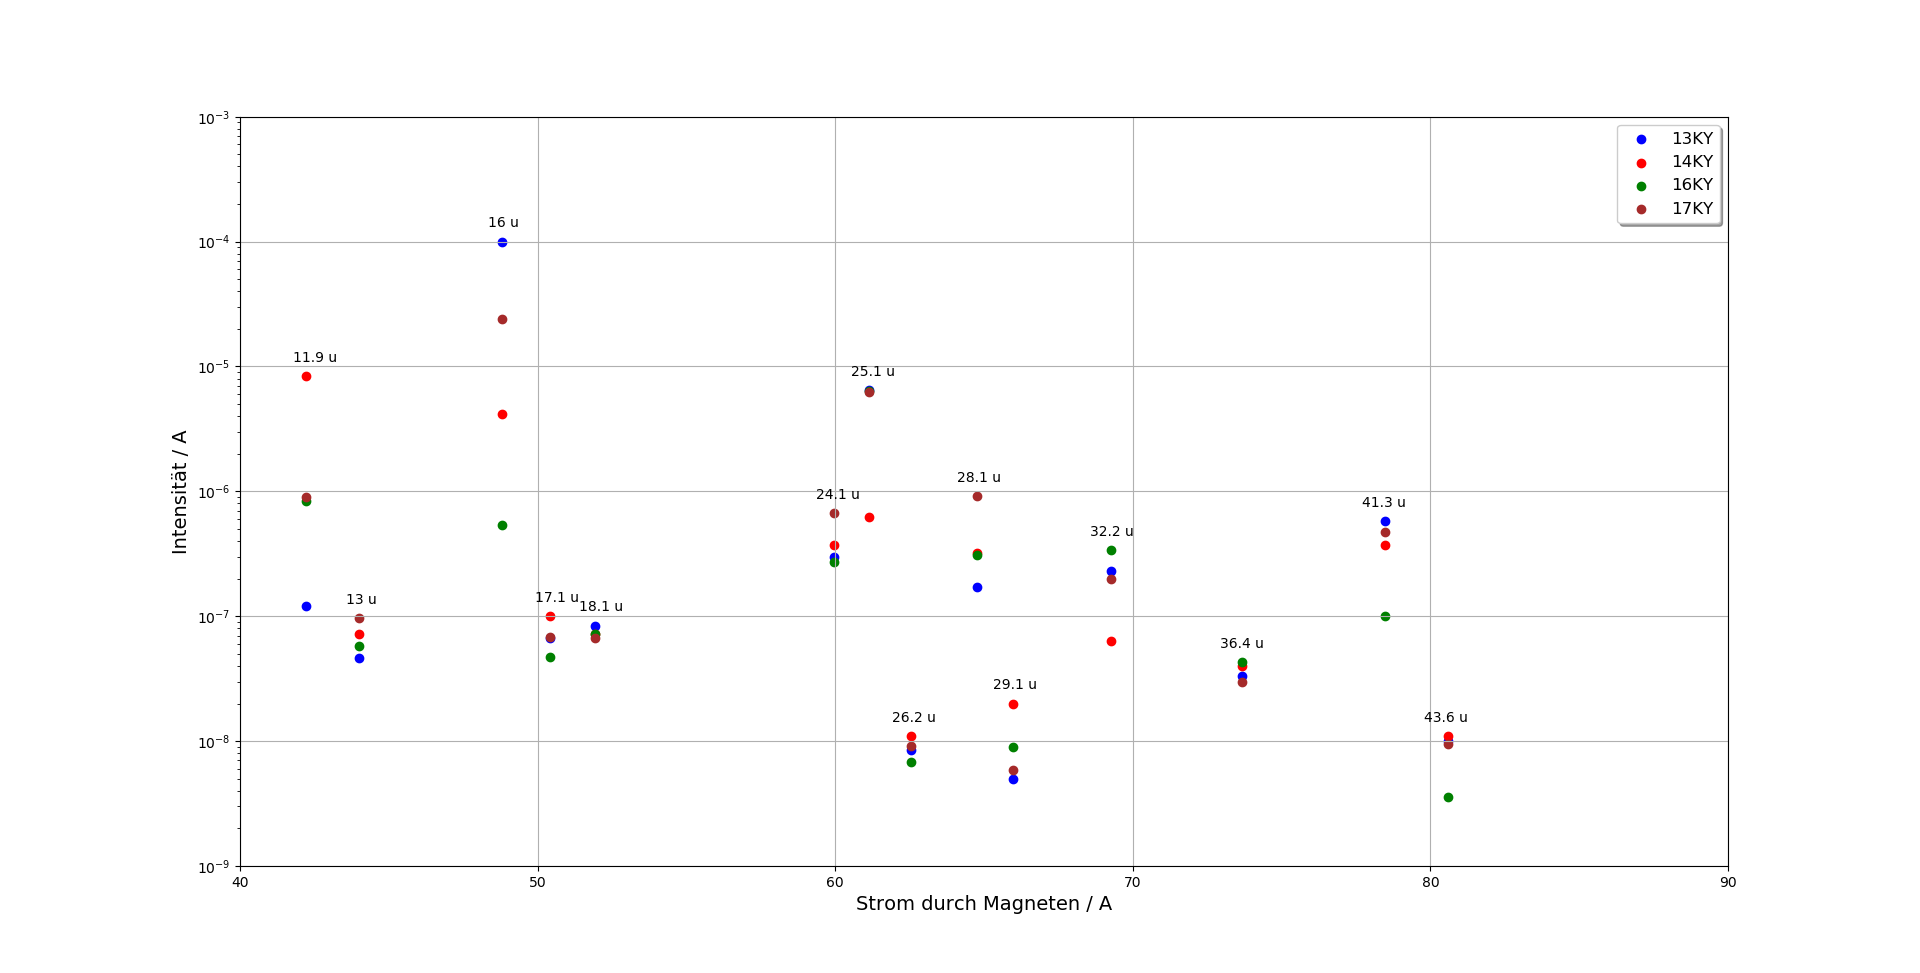
\includegraphics[width=.95\linewidth]{../Pictures/LE_samples_current.png}
\caption{Gemessene Intensitäten für die KY Proben in abhängigkeit der Stromstärke am Magneten.}
\end{subfigure} \quad
\vskip\baselineskip
\begin{subfigure}{\textwidth}
\centering
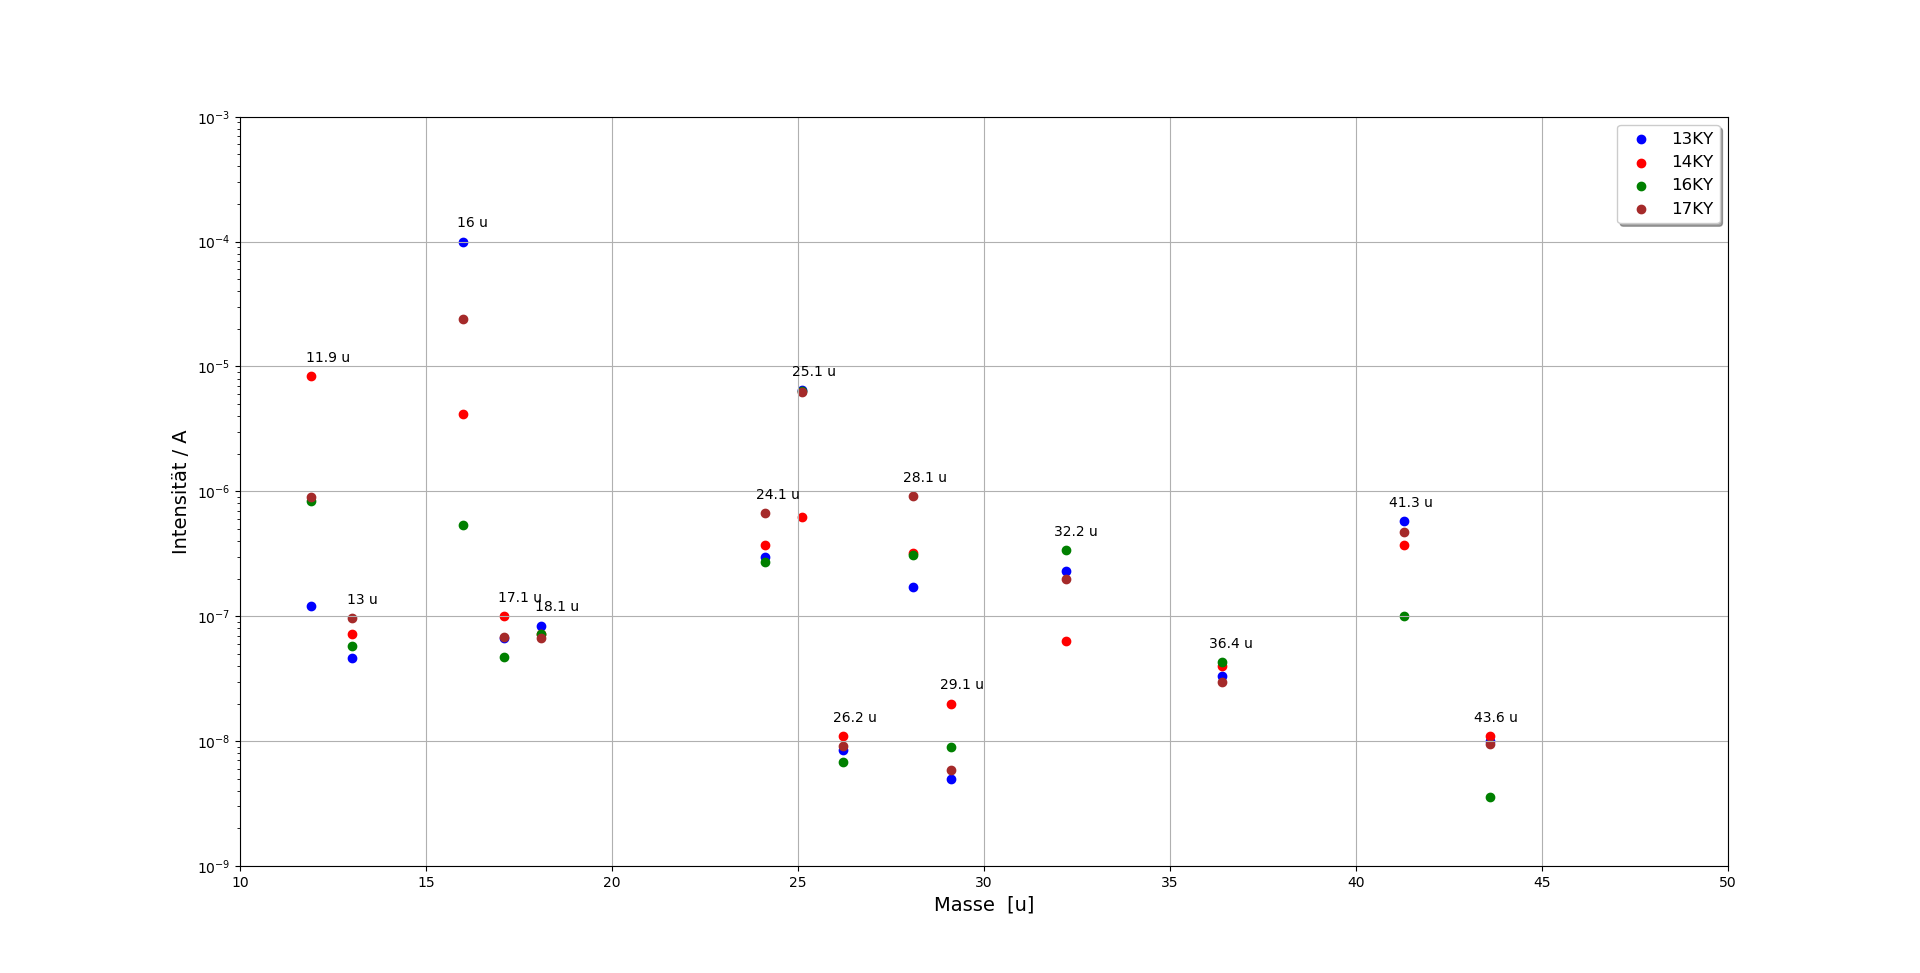
\includegraphics[width=.95\linewidth]{../Pictures/LE_samples_mass.png}
\caption{Probe 153BeO}
\end{subfigure}
\caption{Gemessene Intensitäten für die KY Proben in abhängigkeit der zugeordneten Masse.}
\label{lowenergy}
\end{figure}

\clearpage

\subsection{Teilchenenergien nach dem Beschleuniger}
Die vorselektierten Ionen werden im ersten Teil des Beschleunigers mit der angelegten Spannung beschleunigt.
In der Mitte treffen sie auf Argon an welchem sie sich umladen und die Moleküle aufbrechen.
(Das Aufbrechen der Moleküle ist kein Problem, da chemische Bindungsenergien typischerweise im \si{\electronvolt}-Bereich liegen, die Ionen bis dahin aber schon mehrere \si{\mega\electronvolt} an kinetischer Energie haben.)
Die entstandenen Ionen werden dann mit ihrer positiven Ladung noch ein weiteres Mal mit der angelegten Spannung beschleunigt (s. Gleichung \ref{Theo_Energie_nach_Beschleuniger}).

In unserem Versuch betrug die Spannung des Beschleunigers \SI{5.2479e6}{\volt}.
Damit ergeben sich für entstandene Ionen eine Energie nach dem Beschleuniger von:
\begin{center}
  \begin{tabular}{|c|c|}
    \hline
    Ion & Energie / \si{\mega\electronvolt} \\
    \hline
    $^{9}\text{Be}^{1+}$ & \num{7.15} \\
    $^{9}\text{Be}^{2+}$ & \num{12.40} \\
    $^{9}\text{Be}^{3+}$ & \num{17.64} \\
    $^{9}\text{Be}^{4+}$ & \num{22.89} \\
    \hline
    $^{10}\text{Be}^{1+}$ & \num{7.28} \\
    $^{10}\text{Be}^{2+}$ & \num{12.53} \\
    $^{10}\text{Be}^{3+}$ & \num{17.77} \\
    $^{10}\text{Be}^{4+}$ & \num{23.02} \\
    \hline
    $^{16}\text{O}^{1+}$ & \num{8.50} \\
    $^{16}\text{O}^{2+}$ & \num{13.74} \\
    $^{16}\text{O}^{3+}$ & \num{18.99} \\
    $^{16}\text{O}^{4+}$ & \num{24.24} \\
    \hline
  \end{tabular}
  \captionof{table}{Ionenenergien nach dem Beschleuniger für ausgewählte Ionen. Es wurde angenommen, dass die $^{16}$O Ionen aus $^{10}$Be$^{16}$O stammen.}
  \label{Auswertung_tab_Ionenenergien_nach_Besch}
\end{center}

Zu beachten ist hier, dass $^9$Be aus $^{9}$Be$^{16}$O stammt und $^{10}$Be aus $^{10}$Be$^{16}$O.
$^{16}$O kann daher prinzipiell von beiden Molekülen stammen.
Sauerstoffionen die von $^{9}$Be$^{16}$O stammen haben dabei eine um ca. $110$ keV höhere Energie, sind, sollten aber auch nur einen entsprechend geringen Anteil ausmachen.

\subsection{Faraday-Cups}
Nachdem wir nun Ionen mit hoher Geschwindigkeit nach dem Beschleuniger haben können wir versuchen, häufig auftretende Nuklide nachzuweisen.
Aufgrund der hohen Anteile dieser Nuklide im Telichenstrahl entsteht durch sie ein nennenswerter Ladungsstrom der mit Faraday-Cups gemessen werden kann.
Um einzelne Ionsorten detektieren zu können ist nach dem Beschleuniger ein \ang{90} Ablenkmagnet angebracht, der funktioniert, wie der auf der Niederenergieseite.
Im Faraday-Cup werden dann die auftreffenden Ströme gemessen, die bei einem bestimmten Strom durch die Spule durch die abgelenkten Ionen entsteht.
Zunächst wollen wir sehen ob sich die Nuklide unserer BeO-Probe nachweisen lassen.
Dafür wurde in Abb. \ref{Auswertung_Bild_Faraday_Cup_BeO_HE} die gemessenen Ionenströme über dem Strom durch den Ablenkmagneten aufgetragen.
\begin{figure}[ht]
	\centering
           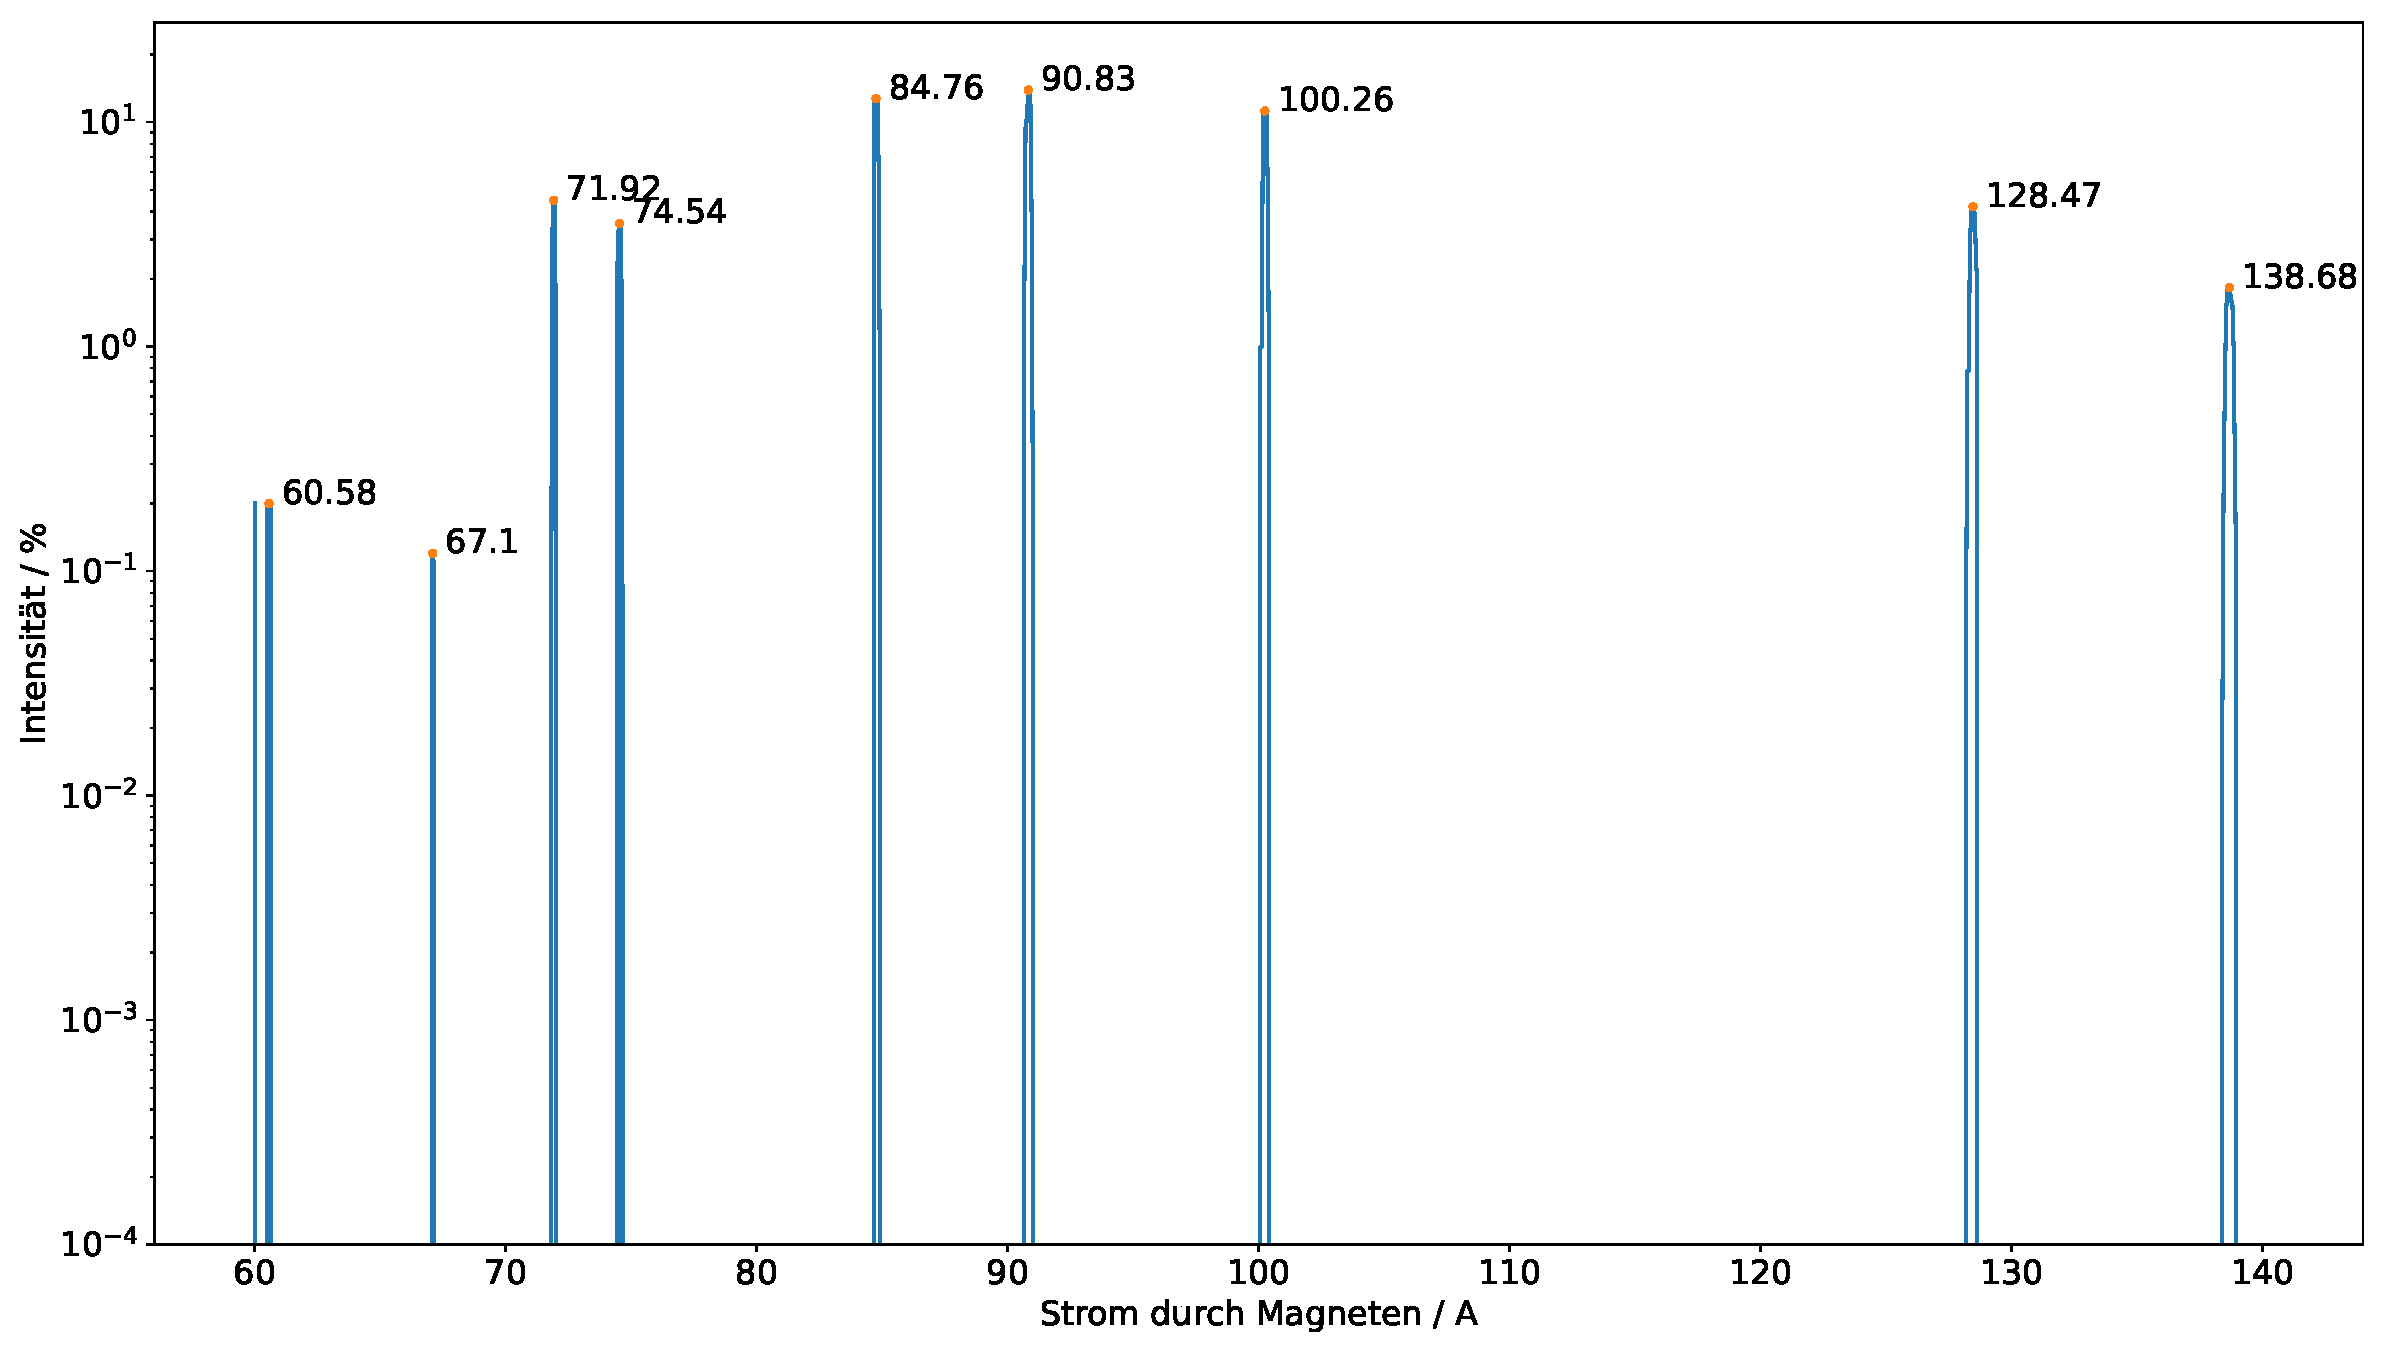
\includegraphics[width=0.85\textwidth]{Pictures/HEMass60-140pos153BeOTUDPract.pdf}
	\caption{Strom gemessen im Faraday-Cup bei variieren des Magnetfeldes auf der Hochenergieseite für BeO-Probe. Die gemittelten x-Werte der Peaks sind eingezeichnet. Die Peaks wurden durch Vergleich mit umliegenden Werten gefunden. Die genaue Position wurde dann ermittelt indem die umliegenden Werte mit ihren Intensitäten als Wichtung gemittelt wurden.}
	\label{Auswertung_Bild_Faraday_Cup_BeO_HE}
\end{figure}

Da durch Massenfilterung nur Teilchen mit der gewählten Masse zu diesem Punkt kommen sollten, wurde für die BeO-Probe folgende Ionen als möglich erachtet:
\begin{center}
  \begin{tabular}{|c|c|c|c|}
    \hline
    Element & Masse $/\ \si{\atomicmassunit}$ & Ladungszustand $/\ e$ & $\frac{\sqrt{m_{\text{ion}}}}{q_{\text{ion}}}$\\
    \hline
    \multirow{8}*{Be}    & \multirow{4}*{$9$}  & $1+$                & \num{3}             \\
                         &                     & $2+$                & \num{1.5}           \\
                         &                     & $3+$                & \num{1}             \\
                         &                     & $4+$                & \num{0.75}          \\
    \cline{2-4}
                         & \multirow{4}*{$10$} & $1+$                & \num{3.16}          \\
                         &                     & $2+$                & \num{1.58}          \\
                         &                     & $3+$                & \num{1.05}          \\
                         &                     & $4+$                & \num{0.79}          \\
    \hline
    \multirow{4}*{O}     & \multirow{4}*{$16$} & $1+$                & \num{4}             \\
                         &                     & $2+$                & \num{2}             \\
                         &                     & $3+$                & \num{1.33}          \\
                         &                     & $4+$                & \num{1}             \\
    \hline
    \multirow{4}*{Al}    & \multirow{4}*{$26$} & $1+$                & \num{5.10}          \\
                         &                     & $2+$                & \num{2.55}          \\
                         &                     & $3+$                & \num{1.70}          \\
                         &                     & $4+$                & \num{1.27}          \\
    \hline
  \end{tabular}
  \captionof{table}{Mögliche Ionen auf Hochenergieseite für BeO-Probe.}
  \label{Auswertung_tab_moegl_ionen}
\end{center}

Mit Formel \ref{Auswertung_eq_Magnet} können wir jetzt wieder über die Verhältnisse der Magnetfelder auf die Ionenmassen schließen.
Dafür ist jedoch zuerst eine Kalibrierung des Magneten erforderlich.
Um diese durchzuführen wurden verschiedene Stromstärken im erwarteten Arbeitsbereich eingestellt und die entsprechende magnetische Feldstärke gemessen.
Mit den so gewonnen Punkten wurde ein linearer Fit durchgeführt, der uns die Kalibriergerade gab.
Die Messdaten und Kurve sind in Abb. \ref{Magnet_kali} zu sehen, die Gerade ergab sich zu:
\begin{equation}
B(I) = ( [\num{6.9} \pm \num{1.3}] + [\num{5.498} \pm \num{0.012}] \cdot I ) \; \si{\milli\tesla}.
\label{kali}
\end{equation}

\begin{figure}[ht]
  \centering
  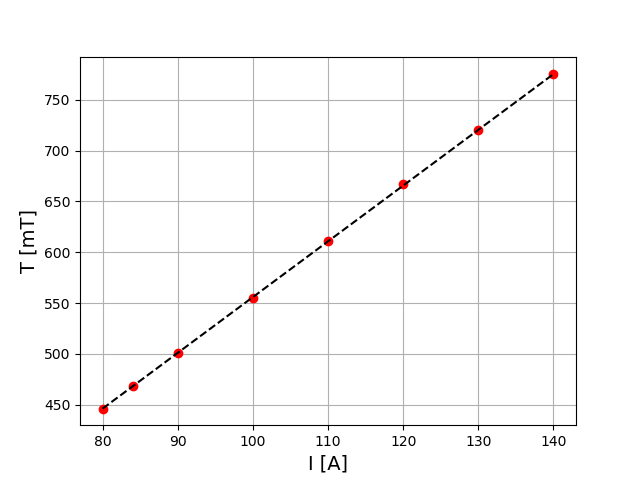
\includegraphics[width=0.95\linewidth]{Pictures/magnet.png}
  \caption{Kalibriergerade des Dipolmagneten.}
  \label{Magnet_kali}
\end{figure}

Mit Kenntnis des Magnetfeldes, sowie der Energie, Masse und Ladung der Teilchen ist es uns jetzt möglich die erwartete Stromstärke für alle Ionen zu berechnen.
Diese folgt aus den Formeln \ref{Auswertung_eq_Magnet} und \ref{kali} zu;
\begin{equation}
I(E, m, q) = \frac{\frac{{\sqrt{2mE}}}{qr}-\num{6.9}}{\num{5.498}}
\label{HE_ion}
\end{equation}
Als Unsicherheit betrachten wir bei dieser Rechnung nur die Unsicherheit der Fitparameter.
Unsicherheiten durch Hysterese an den Magneten sollten zwar einen Enfluss haben, wird aber hier nicht beachtet da keine passende Messung durchgeführt wurde.

Nun ist es möglich den Messpunkt eines bekannten Ions, in diesem Fall $^{10}$Be$^{2+}$, einzusetzen, welches im Faraday-Cup gemessen wird.
Völlig analog zur Niedrigenergieseite ergibt sich das Magnetfeld hier zu $B \rho = \frac{p}{q} = \frac{\sqrt{2mE}}{q}$, mit dem Radius des Magneten $\rho = \SI{1.5}{\metre}$ m.
Für $^{10}$Be$^{2+}$ ergibt sich damit mit der Energie nach Beschleunigung von $E = \SI{12.5}{\mega\electronvolt}$: $B = \SI{537}{\milli\tesla}$.
Mit Formel \ref{kali} ergibt sich damit für die Stromstärke für $^{10}$Be$^{2+}$: $I = \SI{96.4}{\ampere}$, was uns wieder als Ausgangspunkt zur Identifikation des Strahls dient.
Die Masse für gemessene Stromstärken ergibt sich jetzt zu:
\begin{equation}
m_2 = m_1 \cdot \left( \frac{B_2}{B_1} \right)^2 = \SI{10}{\atomicmassunit} \cdot \left( \frac{I}{\SI{96.4}{\ampere}} \right)^{2}
\end{equation}
Die so berechneten Massen sind in Tab. \ref{highenergy} zu sehen.
Durch betrachten der möglichen Verhältnisse von Ladung und Masse sowie Vergleich mit $^{10}$Be$^{2+}$ konnten dann die Teilchen identifiziert werden.
Zu beachten ist hier einerseits, dass wir nach dem Tandem eine vielzahl von Ladungszuständen erwarten und dass wir von einem Ion mit zweifach negativer Ladung ausgehen.
Auch zu beachten ist, dass wir die Messgenauigkeiten (z. B. Hystereseeffekte beim Magneten) hier nicht kennen, weshalb hier eine gewisse Abweichung zu erwarten ist.

\begin{table}[h]
\centering
\caption{Berechnung der Massen im Hochenergiebereich für Probe 153Be.}
\begin{tabular}{|c |c| c|}
\hline
I / \si{A} & m / \si{\atomicmassunit} & Ion \\
\hline
\num{60.5}   & \num{4.0}  &  $^{12}$C$^{2+}$  \\
\num{67.1}   & \num{4.9}  &  $^{10}$Be$^{4+}$ \\
\num{71.92}  & \num{5.6}  &  $^{9}$Be$^{3+}$  \\
\num{74.54}  & \num{6.0}  &  $^{10}$Be$^{3+}$ \\
\num{84.76}  & \num{7.4}  &  $^{16}$O$^{4+}$  \\
\num{90.83}  & \num{8.9}  &  $^{9}$Be$^{2+}$  \\
\num{100.26} & \num{10.8} &  $^{26}$Al$^{4+}$ \\
\num{128.47} & \num{17.7} &  $^{16}$O$^{2+}$  \\
\num{138.68} & \num{20.7} &  $^{9}$Be$^{1+}$  \\
\hline
\end{tabular}
\label{highenergy}
\end{table}

Dabei ist zu beachten, dass $^{10}\text{B}$ nicht von $^{10}\text{Be}$ unterschieden werden kann und es daher auch keinen Sinn macht es mit aufzunehmen.
Isobare können erst im weiteren Verlauf getrennt werden.
Das Vorhandensein von $^{26}$Al$^{4+}$ lässt sich damit erklären, dass dieses aufgrund seiner Masse bisher nicht magnetisch herausgefiltert wurde.
Wie bereits im Niedrigenergiebereich erwähnt, ist dieses schwer vom BeO zu trennen.
Nicht beachtet wurden hier die verschiedenen Sauerstoffisotope, da diese relativ selten selten sind.
Prinzipiel wäre es durch Kentnis des Magneten mit den Formeln \ref{Auswertung_eq_Magnet} und \ref{kali} auch möglich direkt die erwartete Stromstärke eines Ions zu berechnen und durch vergleich der erwarteten mit den berechneten auf die Ionen zu schließen.
Dabei wäre es jedoch nachteilig, dass ohne Verhältnisbildung die Unsicherheiten der Messung weniger eliminiert werden, welche uns nicht bekannt sind.

\clearpage

\subsection{Isobarentrennung}
Wie in dem vorherigen Abschnitt bereits erwähnt ist es bis hierhin noch nicht möglich gewesen Isobare zu unterscheiden.
Um Abhilfe zu schaffen ist im weiteren Strahlenverlauf eine dünne Schicht aus Siliziumnitrid angebracht.
Da der Verlust an kinetischer Energie von Atomen in Materie stark von der Kernladungszahl abhängt erlaubt dies die Isobarentrennung.
den Faktor $\frac{\Delta E}{\Delta x}$ erhalten wir aus der frei verfügbaren Software SRIM.
Die SiN-Folie hat eine Dicke von \SI{1}{\micro\metre}.
Die verbleibende Energie der $^{10}\text{Be}$-Ionen un der $^{10}\text{B}$-Ionen ist dann, abhängig von deren Energie vorher:
\begin{center}
  \begin{tabular}{|c|c|c|c|}
    \hline
    Ion & Energie nach Beschleuniger & $\frac{\Delta E}{\Delta x}$ & Energie nach Folie \\
    \hline
    $^{10}\text{Be}^{1+}$ & \SI{7.3}{\mega\electronvolt}  & \SI{1053}{\kilo\electronvolt\per\micro\metre} & \SI{6.2}{\mega\electronvolt} \\
    $^{10}\text{Be}^{2+}$ & \SI{12.5}{\mega\electronvolt} & \SI{851}{\kilo\electronvolt\per\micro\metre} & \SI{11.7}{\mega\electronvolt} \\
    $^{10}\text{Be}^{3+}$ & \SI{17.8}{\mega\electronvolt} & \SI{714}{\kilo\electronvolt\per\micro\metre} & \SI{17.1}{\mega\electronvolt} \\
    $^{10}\text{Be}^{4+}$ & \SI{23.0}{\mega\electronvolt} & \SI{621}{\kilo\electronvolt\per\micro\metre} & \SI{22.4}{\mega\electronvolt} \\
    \hline
    $^{10}\text{B}^{1+}$ & \SI{7.3}{\mega\electronvolt}  & \SI{1449}{\kilo\electronvolt\per\micro\metre} & \SI{5.8}{\mega\electronvolt} \\
    $^{10}\text{B}^{2+}$ & \SI{12.5}{\mega\electronvolt} & \SI{1227}{\kilo\electronvolt\per\micro\metre} & \SI{11.3}{\mega\electronvolt} \\
    $^{10}\text{B}^{3+}$ & \SI{17.8}{\mega\electronvolt} & \SI{1052}{\kilo\electronvolt\per\micro\metre} & \SI{16.7}{\mega\electronvolt} \\
    $^{10}\text{B}^{4+}$ & \SI{23.0}{\mega\electronvolt} & \SI{925}{\kilo\electronvolt\per\micro\metre} & \SI{22.1}{\mega\electronvolt} \\
    \hline
  \end{tabular}
  \captionof{table}{Ionenenergien nach der SiN Folie in Abhängigkeit der Ladungszustände aus dem Beschleuniger.}
  \label{Auswertung_tab_Ionenenergien_nach_Folie}
\end{center}
Nach der Folie wird $^{10}\text{Be}$ nur noch im Ladungszustand $4+$ erwartet, da die Atome durch die Foile weiter ionisiert werden.

Um nun die Isobare $^{10}\text{Be}$ und $^{10}\text{B}$ zu trennen ist nach der Folie ein elektrostatischer Analysierer angebracht.
Die Spannung die angelegt werden muss kann berechnet werden durch Kräftegleichgewicht:
\begin{gather}
    q_{\text{Ion+}} \cdot \frac{U_{\text{Platte}}}{d_{\text{Platte}}} = \frac{mv^{2}}{r}
\end{gather}
Wobei $d_{\text{Platte}} = \SI{3.6}{\centi\metre}$ und $r = \SI{2.6}{\metre}$ ist.
Die Spannung, die einzustellen ist, ist jedoch nur die halbe, da auf den Platten jeweils $+U_{\text{Platte}}$ und $-U_{\text{Platte}}$ erzeugt wird (die Spannung wird beim einstellen relativ zur Erdung gemessen).
Für das Ion $^{10}\text{Be}^{4+}$ ergibt sich daher in Abhängigkeit der Energie nach der Folie eine Ablenkspannung von:
\begin{center}
  \begin{tabular}{|c|c|c|}
    \hline
    Ion & Energie nach Folie & $\frac{U_{\text{Platte}}}{2}$ \\
    \hline
    \multirow{4}*{$^{10}\text{Be}^{4+}$} & \SI{6.2}{\mega\electronvolt}  & \SI{21.5}{\kilo\volt} \\
                                         & \SI{11.7}{\mega\electronvolt} & \SI{40.4}{\kilo\volt} \\
                                         & \SI{17.1}{\mega\electronvolt} & \SI{59.1}{\kilo\volt} \\
                                         & \SI{22.4}{\mega\electronvolt} & \SI{77.5}{\kilo\volt} \\
    \hline
  \end{tabular}
  \captionof{table}{Ablenkspannug für den ESA für verschiedene Ionenenergien.}
  \label{Auswertung_tab_Ablenkspannung_ESA}
\end{center}

\subsection{Gasgefüllter Ionisationsdetektor}
Im letzten Schritt treffen die verbliebenen Ionen in den Ionisationsdetektor ein, der mit Isobutan ($C_{4}H_{10}$) gefüllt ist.
Auch hier verlieren die Ionen wieder Energie beim durchqueren des Mediums.
Dadurch ionisieren sie das Isobutan.
Die entstandenen freien Ladungsträger werden durch das elektrische Feld abgesaugt und führen zu einem detektierbaren Strom.
Die Dichte des Isobutan wurde mit der thermischen Zustandsgleichung idealer Gase abgeschätzt:
\begin{gather}
    \rho = \frac{p \cdot m}{k_{B} \cdot T}
\end{gather}
Wobei $k_{B}$ die Boltzmann-Konstante ist.
Der Druck $p$ war angegeben mit \SI{31.0e-3}{\bar}, die Temperatur $T$ mit \SI{21.0}{\degreeCelsius} und die Masse eines Isobutan-Moleküls $m$ ist etwa \SI{58}{\atomicmassunit}.
Damit ergibt sich eine Dichte von \SI{7e-5}{\gram\per\cubic\centi\metre}.
Mithilfe von SRIM/TRIM lassen sich nun wieder die Abbremsungen ermitteln.
Die durch die Monte-Carlo-Simulation erhaltenen Eindringtiefen befinden sich in Tabelle \ref{Auswertung_tab_Gasdetektor_Eindringtiefen}.
\begin{table}[H]
  \centering
  \caption{Eindringtiefe der Ionen in Isobutan mit Dichte $\rho = \SI{7e-5}{\gram\per\cubic\centi\metre}$. Bor ist mit aufgenommen um zu untersuchen ob das Isobar vollständig beseitigt werden konnte. Da der Detektor nur eine Länge von etwa \SI{30}{\centi\metre} hat würden einige Ionen den Detektor wieder verlassen. Die Eindringtiefe wurde mithilfe von SRIM/TRIM ermittelt.}
  \begin{tabular}{|c|c|c|}
    \hline
    Ion (nach Folie) & Energie nach Folie & Eindringtiefe in Isobutan \\
    \hline
    \multirow{4}*{$^{10}\text{Be}^{4+}$} & \SI{6.22}{\mega\electronvolt}  & \SI{146}{\milli\metre} \\
                                         & \SI{11.67}{\mega\electronvolt} & \SI{284}{\milli\metre} \\
                                         & \SI{17.06}{\mega\electronvolt} & \SI{467}{\milli\metre} \\
                                         & \SI{22.40}{\mega\electronvolt} & \SI{693}{\milli\metre} \\
    \hline
    \multirow{4}*{$^{10}\text{B}^{4+}$}  & \SI{5.83}{\mega\electronvolt}  & \SI{102}{\milli\metre} \\
                                         & \SI{11.30}{\mega\electronvolt} & \SI{200}{\milli\metre}    \\
                                         & \SI{16.72}{\mega\electronvolt} & \SI{324}{\milli\metre}    \\
                                         & \SI{22.10}{\mega\electronvolt} & \SI{476}{\milli\metre}    \\
    \hline
  \end{tabular}
  \label{Auswertung_tab_Gasdetektor_Eindringtiefen}
\end{table}
Mit den Eindringtiefen wird klar, dass $^{10}\text{Be}$, welches nach der Mitte des Tandems einen Ladungszustand von $3+$ oder mehr hatte durch den Detektor durchfliegen würde.
Es bietet sich daher für die Messung an $^{10}\text{Be}^{2+}$ Ionen auszuwählen (Den Magneten nach dem Beschleuniger darauf einstellen; Magnet und ESA nach der Folie werden auf den ladungszustand $4+$ eingestellt).
Dies wurde in den aufgenommenen Spektren getan.
In den Abbildungen \ref{Auswertung_Gasdetektor_2DSpektren_blank}, \ref{Auswertung_Gasdetektor_2DSpektren_BeO} und \ref{Auswertung_Gasdetektor_2DSpektren_unbekannt} sind diese für verschiedene Proben zu finden.
\begin{figure}[H]
    \centering
    \begin{subfigure}{0.47\textwidth}
        \centering
        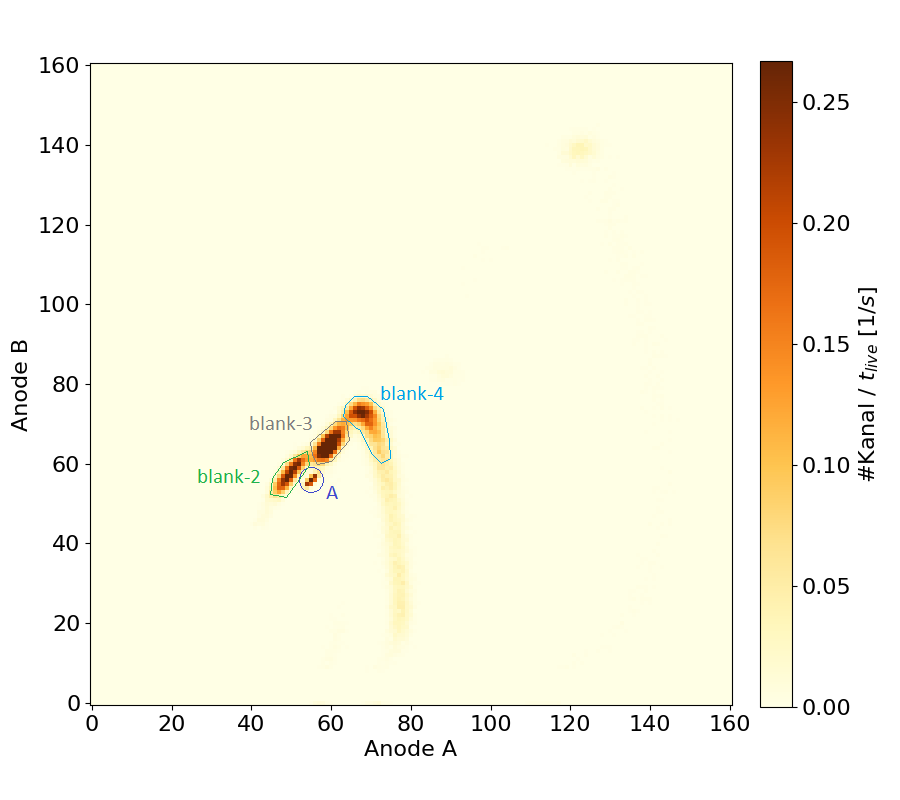
\includegraphics[width=\linewidth]{Pictures/Gasdetektor/3_blank_AB.png}
    \end{subfigure}
    \begin{subfigure}{0.47\textwidth}
        \centering
        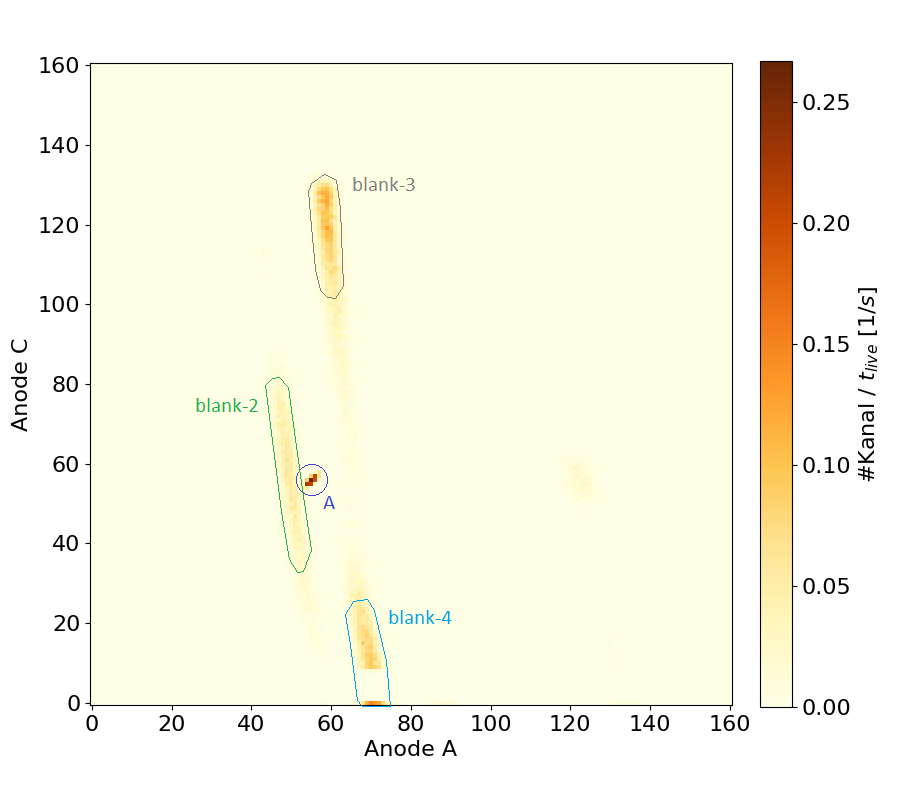
\includegraphics[width=\linewidth]{Pictures/Gasdetektor/3_blank_AC.png}
    \end{subfigure}
    \begin{subfigure}{0.47\textwidth}
        \centering
        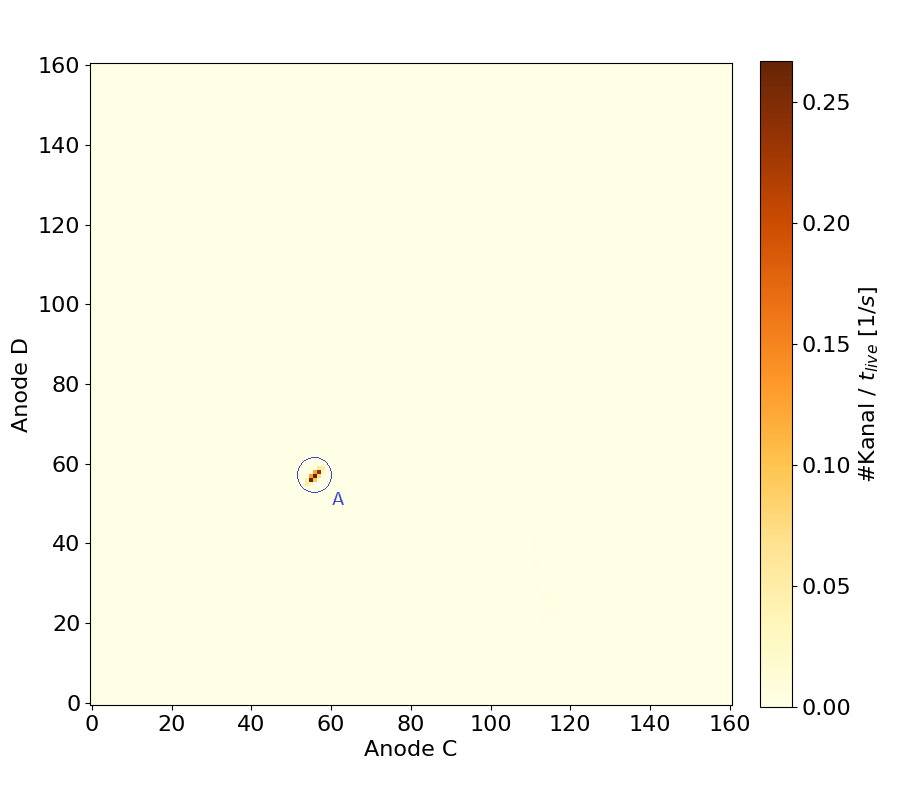
\includegraphics[width=\linewidth]{Pictures/Gasdetektor/3_blank_CD.png}
    \end{subfigure}
    \caption{2D-Spektren der Anoden in der Gasionisationskammer ohne Probe, live-Zeit von $t_{\text{live}} = \SI{1245}{\second}$}
    \label{Auswertung_Gasdetektor_2DSpektren_blank}
\end{figure}
\begin{figure}[H]
    \centering
    \begin{subfigure}{0.47\textwidth}
        \centering
        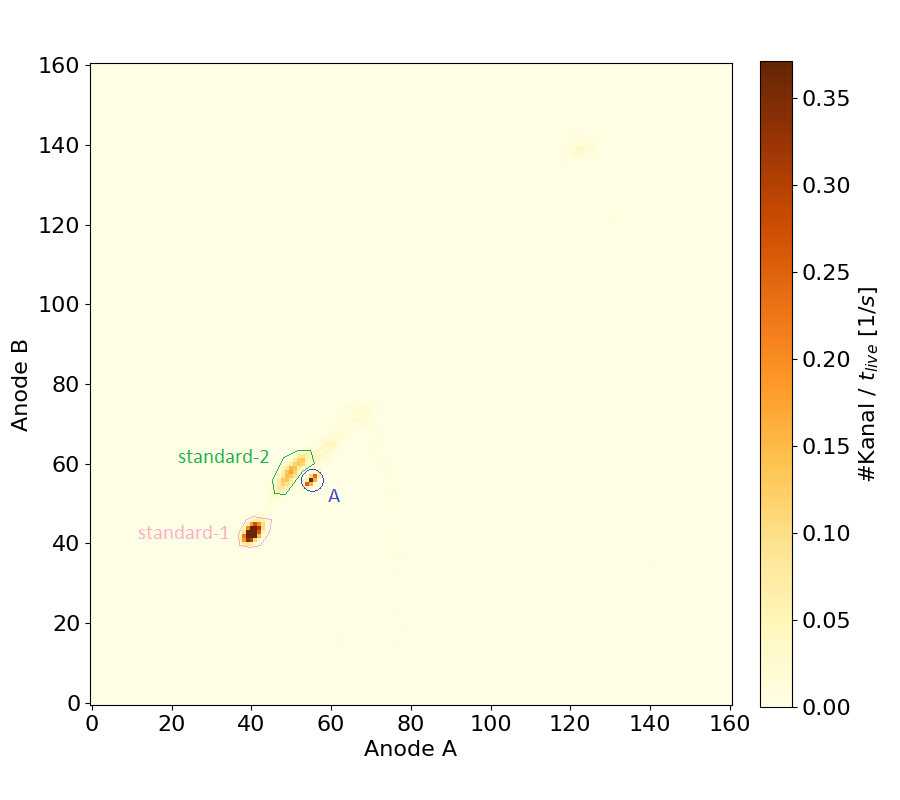
\includegraphics[width=\linewidth]{Pictures/Gasdetektor/22_standard_AB.png}
    \end{subfigure}
    \begin{subfigure}{0.47\textwidth}
        \centering
        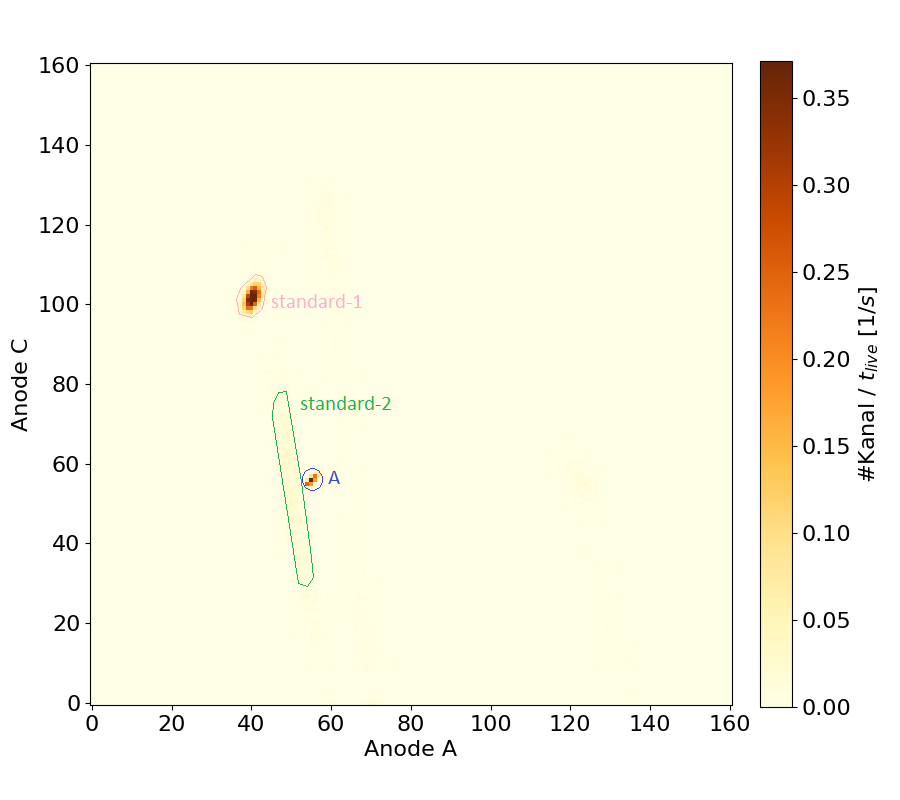
\includegraphics[width=\linewidth]{Pictures/Gasdetektor/22_standard_AC.png}
    \end{subfigure}
    \begin{subfigure}{0.47\textwidth}
        \centering
        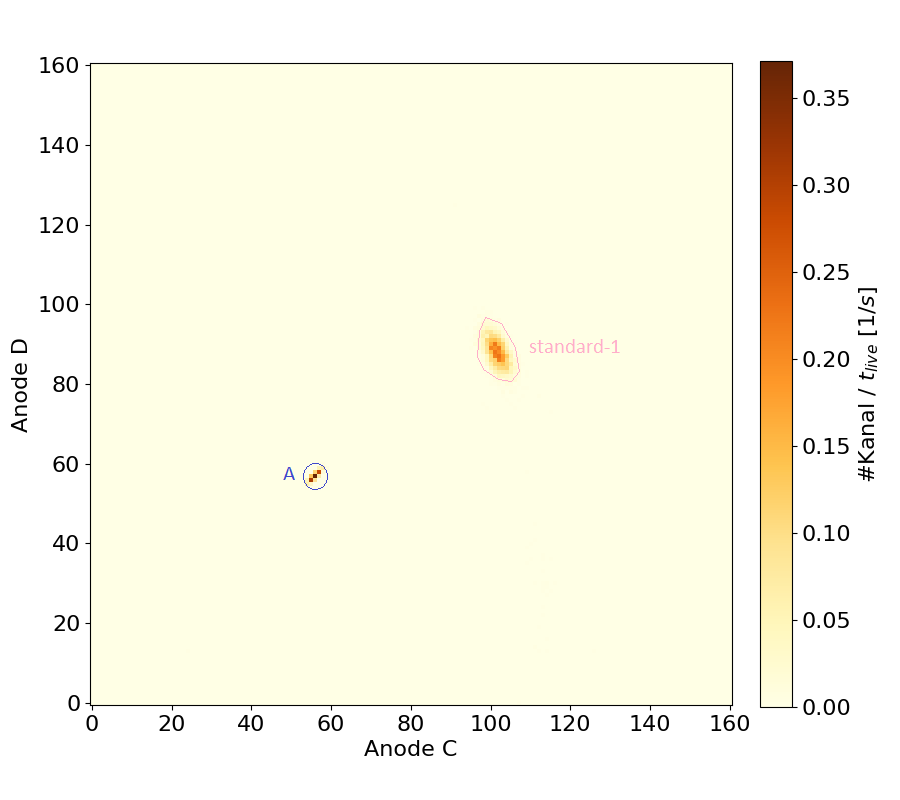
\includegraphics[width=\linewidth]{Pictures/Gasdetektor/22_standard_CD.png}
    \end{subfigure}
    \caption{2D-Spektren der Anoden in der Gasionisationskammer mit BeO-Probe, live-Zeit von $t_{\text{live}} = \SI{474}{\second}$}
    \label{Auswertung_Gasdetektor_2DSpektren_BeO}
\end{figure}
\begin{figure}[H]
    \centering
    \begin{subfigure}{0.47\textwidth}
        \centering
        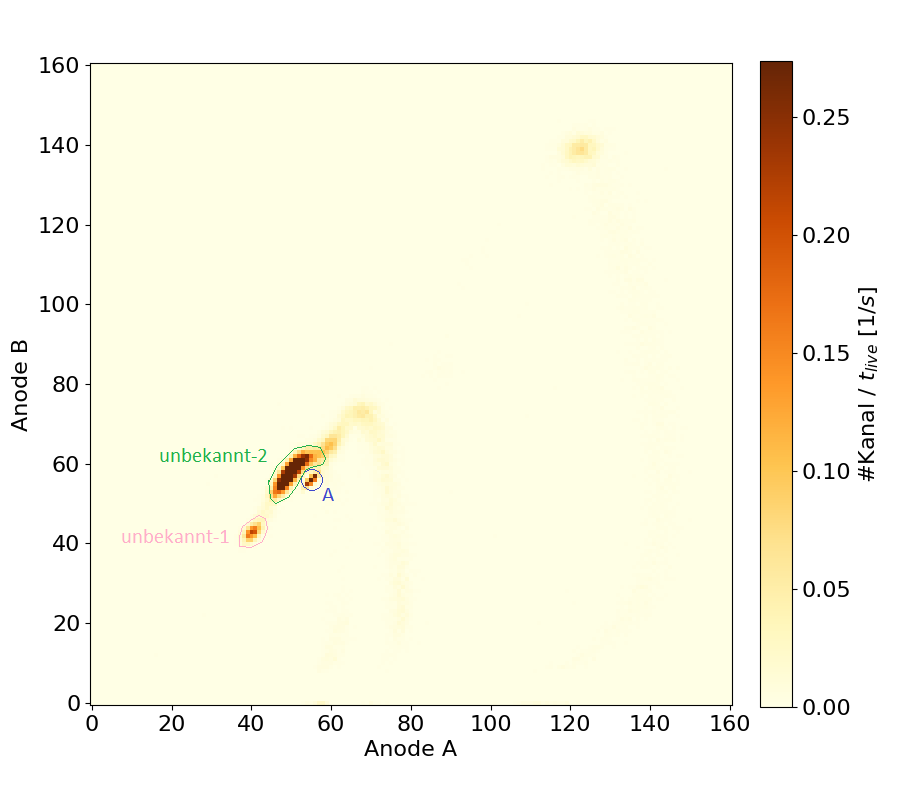
\includegraphics[width=\linewidth]{Pictures/Gasdetektor/19_probe_AB.png}
    \end{subfigure}
    \begin{subfigure}{0.47\textwidth}
        \centering
        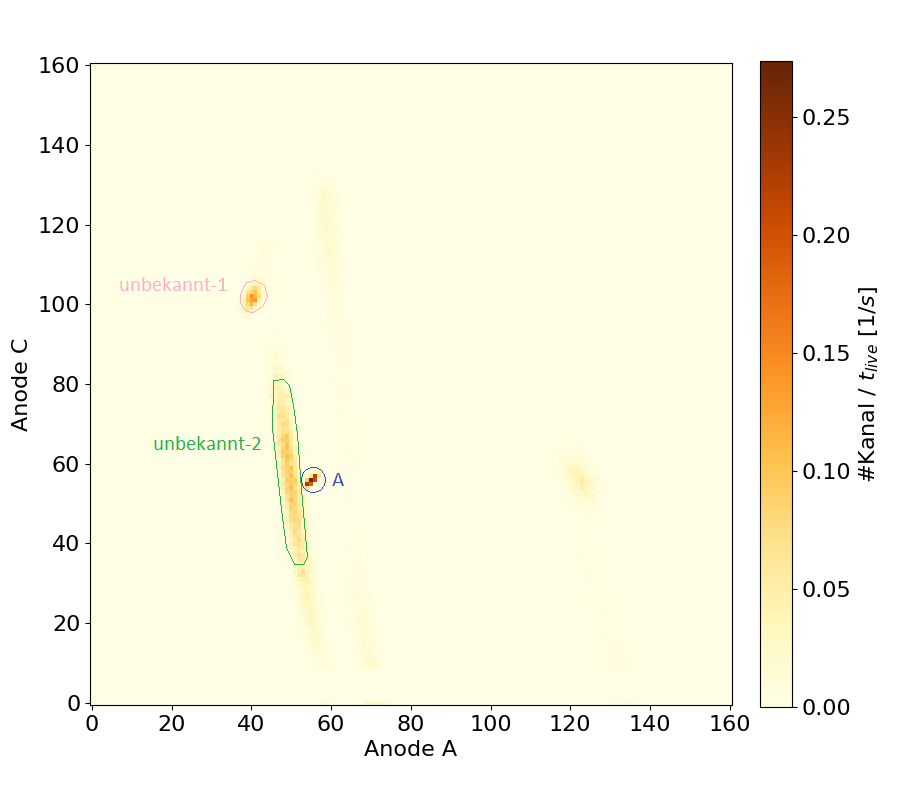
\includegraphics[width=\linewidth]{Pictures/Gasdetektor/19_probe_AC.png}
    \end{subfigure}
    \begin{subfigure}{0.47\textwidth}
        \centering
        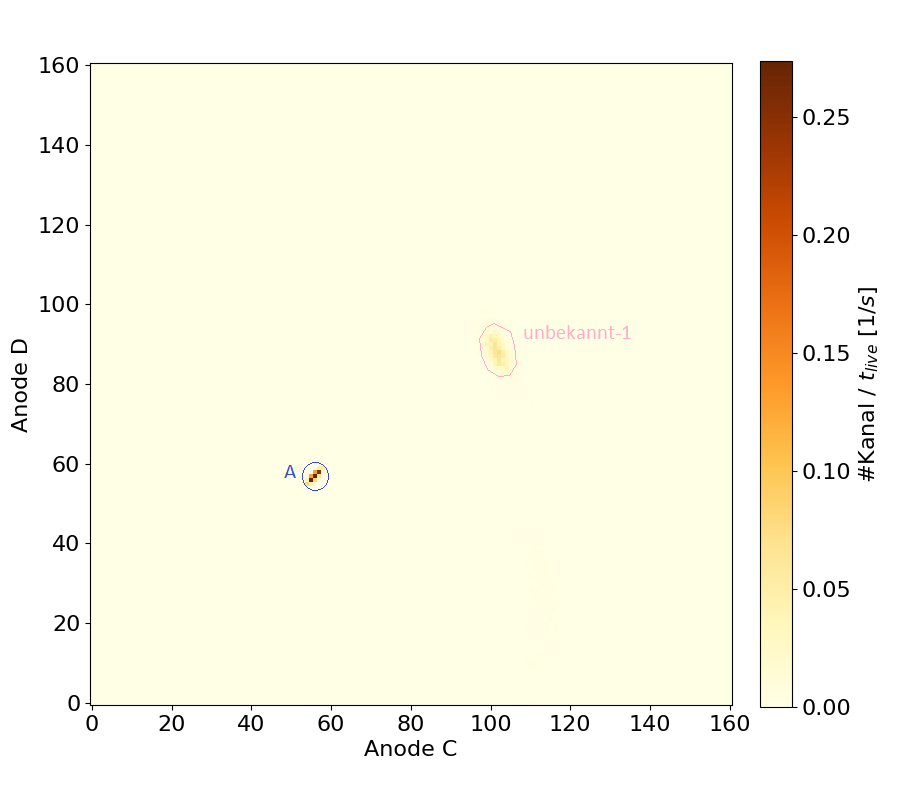
\includegraphics[width=\linewidth]{Pictures/Gasdetektor/19_probe_CD.png}
    \end{subfigure}
    \caption{2D-Spektren der Anoden in der Gasionisationskammer mit unbekannter Probe, live-Zeit von $t_{\text{live}} = \SI{845}{\second}$}
    \label{Auswertung_Gasdetektor_2DSpektren_unbekannt}
\end{figure}
Um die Markierten Bereiche etwas besser zu verstehen sind im Folgenden noch zwei TRIM-Simulationen visualisiert, bei denen die Ionisierung des Isobutan über der Eindringtiefe zweier Ionen aufgetragen ist:
\begin{figure}[H]
    \centering
    \begin{subfigure}[t]{0.47\textwidth}
        \centering
        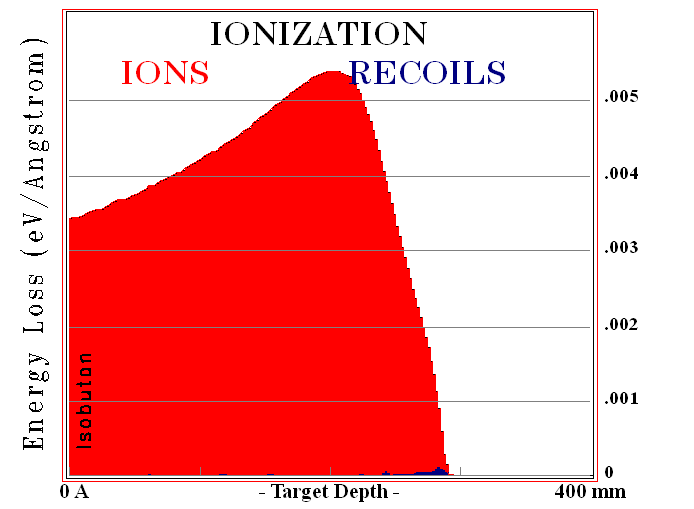
\includegraphics[height=0.25\textheight]{Pictures/TRIM_Ionisierung_10Be_in_Isobutan_vorher_2+.png}
        \caption{TRIM-Simulation für die Ionisierung von Isobutan durch $^{10}\text{Be}$, mit Anfangsenergie $E_{\text{Ion, Start}} = \SI{11.67}{\mega\electronvolt}$ (vor Folie $^{10}\text{Be}^{2+}$)}
        \label{Auswertung_Gasdetektor_TRIM_sims_Be}
    \end{subfigure}
    \begin{subfigure}[t]{0.47\textwidth}
        \centering
        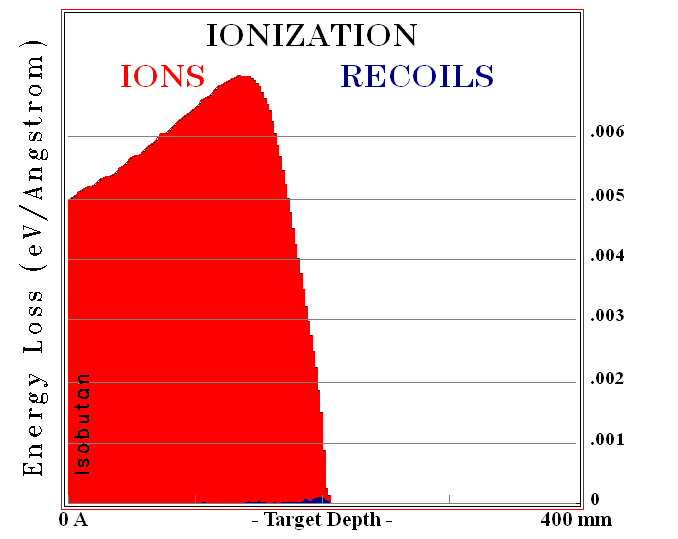
\includegraphics[height=0.25\textheight]{Pictures/TRIM_Ionisierung_10Bor_in_Isobutan_vorher_2+.png}
    	\caption{TRIM-Simulation für die Ionisierung von Isobutan durch $^{10}\text{B}$, mit Anfangsenergie $E_{\text{Ion, Start}} = \SI{11.30}{\mega\electronvolt}$ (vor Folie $^{10}\text{B}^{2+}$)}
        \label{Auswertung_Gasdetektor_TRIM_sims_B}
    \end{subfigure}
    \caption{TRIM-Simulationen für die Ionisierung von Isobutan durch $^{10}\text{Be}$ und $^{10}\text{B}$, wenn sie jeweils nach dem Beschleuniger den Ladungszustand $2+$ und nach der SiN-Folie den Ladungszustand $4+$ haben. Dies sind die einfachsten Fälle von Ionen, die es (möglicherweise) in den Detektor schaffen. Da bei Bor keine Ionisierung im Bereich ab \SI{20}{\centi\metre} stattfindet ist zu erwarten, dass Bor nicht in Spektren auftritt die die C- und D-Anode übereinander auftragen, solange das Bor mit der Anfangsenergie $E_{\text{Ion, Start}} = \SI{11.30}{\mega\electronvolt}$ eintrifft.}
    \label{Auswertung_Gasdetektor_TRIM_sims}
\end{figure}
Die Fläche unter den Ionisierungskurven bis zu einer bestimmten Eindringtiefe bestimmt den Ort des Ions in den 2-D-Spektren.

Fangen wir bei der Auswertung mit den Gemeinsamkeiten der Spektren an.
Für die Auswertung wurden ähnliche Bereiche in den Spektren mit den selben Nummern und Farben versehen.
Man kann die selbe Teilchenspezies über zwei Spektren hinweg miteinander identifizieren, da immer mindestens eine Achse zwischen den Spektren geteilt ist, und Spezies auf einer Achse (wenn überhaupt) in jedem Spektrum in dem selben Wertebereichen stehen müssen.
Daher sind die Farben und Nummern in allen Spektren geteilt, und man sieht das im wesentlichen fünf verschiedene Spezies identifiziert werden müssen.
Dabei muss nicht jedes ein neues Nuklid sein, es kann sich auch um ein schon gefundenes Nuklid handeln, welches aber eine andere Anfangsenergie besitzt.

Zuerst schauen wir uns die bekannte BeO-Probe in Abb. \ref{Auswertung_Gasdetektor_2DSpektren_BeO} an.
Da wir in der BeO-Probe davon ausgehen können eine sehr reine Probe zu haben, ist der Bereich 1 (pink) eindeutig dem Nuklid $^{10}Be$ zuzuordnen, denn es tritt am häufigsten auf und es wird in allen Spektren in sinnvollen Kanälen gefunden (Kanäle entsprechen dabei dem Strom, und damit der Energie die an einer Anode ankam).
Man kann also davon ausgehen, dass dieses $^{10}\text{Be}$ aus der Probe als $^{10}\text{Be}^{16}\text{O}^{1-}$ gelöst wurde.
Im Tandembeschleuniger ist der Sauerstoff abgespalten und $^{10}\text{Be}^{2+}$ wurde weiter beschleunigt.
In der SiN-Folie wurde es schließlich Umgeladen zu $^{10}\text{Be}^{4+}$, als welches es schließlich in den Detektor gefallen ist.
Da wir die Kalibrierung der ESA und der Ablenkmagnete genau auf diesen Prozess eingerichtet haben hat es kein Problem den Detektor zu erreichen.

Kniffliger wird es bei Spezies 2 (grün), denn diese wird ebenfalls in der reinen BeO-Probe gefunden, jedoch findet man sie dort nicht im Spektrum der letzten beiden Anoden.
Sie schafft es jedoch bis zur Anode C, das heißt sie wird in dieser Detektortiefe vollständig gestoppt.
Da sie schon im Spektrum von Anode A und B erkennbar mehr Energie verliert als Spezies 1, jedoch im Spektrum von Anode A und C unter der Spezies 1 liegt und damit dort weniger Energie abgibt, und wegen der reinen BeO-Probe, liegt es nahe, dass es sich hier auch um Beryllium handelt.
Denn wenn dieses eine niedrigere Energie bei Eintritt in den Detektor (im Vergleich mit Spezies 1) mitbringt ist genau dieses Verhalten zu erwarten.
Der beste Kandidat für diese Spezies ist $^{9}\text{Be}$, denn dieses kann als $^{9}\text{Be}^{16}\text{O}^{1}\text{H}^{1-}$ aus der Probe gelöst werden, kann sich dann im Tandem vom $^{16}\text{O}$ trennen und dann als Isobar $^{9}\text{Be}^{1}\text{H}^{2+}$ bis zur SiN-Folie bewegen.
Das $^{9}\text{Be}^{16}\text{O}^{1}\text{H}^{1-}$ im Tandem nicht auch den Wasserstoff verliert ist unwahrscheinlich.
Dies erklärt immerhin teilweise die geringe Intensität der Spezies in dem Spektrum von BeO (im Vergleich zu $^{10}\text{Be}$, welches sonst deutlich seltener wäre).
Beim Eintritt in die dichte Folie trennen sich $^{9}\text{Be}$ und $^{1}\text{H}$.
Das $^{9}\text{Be}$ verbleibt mit $\frac{9}{10}$ der kinetischen Energie des Ions nach dem Beschleuniger (\SI{11.27}{\mega\electronvolt}).
Dann wird es in der SiN-Folie abgebremst.
Hier wurde wieder SRIM/TRIM benutzt.
Die Energie nach der Folie ist dann \SI{10.42}{\mega\electronvolt}, die Spezies ist $^{9}\text{Be}^{4+}$.
Damit hat es ca. \SI{89}{\percent} der Energie, die ein $^{10}\text{Be}^{4+}$ an dieser stelle hätte, also wie gesucht weniger.
Weitere SRIM/TRIM-Simulationen zeigen, dass es mit dieser Energie eine Eindringtiefe von \SI{254}{\milli\metre} im Detektor hätte, also würde es auch Anode D erreichen.
Was hier jedoch noch fehlt, ist das das Ion aufgrund seiner geringeren kinetischen Energie und Masse nicht ohne Probleme durch den HE-ESA und den vertikalen Ablenkmagneten kommt.
Im ESA führt dies zu einer stärkeren Ablenkung (nach Gleichung \ref{Auswertung_Formel_ESA} ist für diesen Fall der Krümmungsradius der Trajektorie proportional zur kinetischen Energie des Ions), im vertikalen Ablenkmagneten ebenfalls zu einer stärkeren (Gleichung \ref{Auswertung_eq_Magnet}, Krümmungsradius proportional zu $\sqrt{m_{\text{Ion}}E_{\text{kin}}}$).
Da die Ablenkungen senkrecht zueinander stehen sind sie quasi unabhängig voneinander.
Es liegt hier nahe, dass das Ion noch Energie verliert wenn es mit dem inneren des Strahlrohrs kollidiert.
Da der Auftreffwinkel aber klein ist verliert es nicht alle Energie, wie viele andere Ionen.
Ein bisschen ausprobieren in TRIM hat gezeigt, dass $^{9}\text{Be}^{4+}$ unterhalb von etwa \SI{8.5}{\mega\electronvolt} Eintrittsenergie nicht mehr die Anode D erreicht.
Da wir den genauen Aufbau nicht kennen, können wir nicht abschätzen, ob so ein Energieverlust realistisch ist.
Dies würde jedoch nicht nur die das Fehlen des Ions im letzten Spektrum erklären, sondern auch warum der Fleck in den anderen Spektren so viel breiter ist als der der ersten Spezies, denn Stöße sind stochastische Prozesse, was unweigerlich zu so einer "Verschmierung" der Energie führt.

Um dieses Argument noch etwas zu bekräftigen wollen wir uns als nächstes die Spektren in Abbildung \ref{Auswertung_Gasdetektor_2DSpektren_blank} ansehen, bei denen gar keine Probe verwendet wurde.
Auch dort ist diese 2. Spezies zu identifizieren, was für das stabile und häufig vorkommende $^{9}\text{Be}$-Isotop spricht.
Als nächstes wollen wir uns mit den Spezies 3 (grau) und 4 (blau) beschäftigen.
Auch hier fällt auf, dass die Ionen nicht die Anode D erreichen können.
Hier werden beide als $^{10}\text{B}$ identifiziert.
In beiden Fällen handelte es sich nach dem Beschleuniger um $^{10}\text{B}^{2+}$.
Auch hier ist die Begründung im wesentlichen eine Energieverlust durch Kollisionen mit dem Strahlrohr (ohne die selben Argumente nocheinmal anzuführen).
Dennoch gibt es Unterschiede.
So kann man der Spezies 3 das Ion $^{10}\text{B}^{4+}$ nach der SiN-Folie zuordnen.
Da es nach der SiN-Folie eine Energie von \SI{11.30}{\mega\electronvolt} ist der Krümmungsradius der Trajektorie im HE-ESA und im vertikalen Ablenkmagneten nicht viel anders als der von $^{10}\text{Be}^{4+}$, jedoch genug um Kollisionen mit dem Strahlrohr zu verursachen und damit eine Aufweichung des Flecks im Spektrum hervorzurufen.
Der Spezies 4 kann das Ion $^{10}\text{B}^{3+}$ nach der SiN-Folie zugeordnet werden.
Dies führt dazu, dass der Krümmungsradius der Trajektorien in beiden Ablenkern am Ende überproportional größer wird (denn beide sind proportional zum inversen der Ladung).
Das Ion kollidiert dann genau mit der anderen Seite des Strahlgangs.
Am Ende hat Spezies 4 die geringste Energie wenn sie in den Detektor kommt, und einige der Ionen schaffen es nicht mal bis zu Anode C, weshalb der Fleck im A-C-Spektrum nach unten etwas abgeschnitten ist.

Als letztes bleibt die Spezies, die in den Spektren mit "A" betitelt wurde.
Hierbei handelt es sich offenbar um Ionen mit einer derart hohen Energie, dass sie den Detektor einfach passieren.
Ferner ist ihr Energieverlust in allen Berechen des Detektors immer fast konstant, was ebenfalls für eine sehr große kinetische Energie spricht, denn Ionen verlieren in den hier betrachteten Energiebereichen immer die meiste Energie in Materie, wenn sie schon fast stehen.
Da kein "Fingerabdruck" im Detektor hinterlassen wird ist eine Identifikation hier nicht möglich.

Schauen wir zum Abschluss noch auf Abbildung \ref{Auswertung_Gasdetektor_2DSpektren_unbekannt}, Spektren einer unbekannte Probe.
Durch die vorherigen Erkenntnisse lassen sich schnell die Teilchenspezies 1 und 2 erkennen.
Es handelt sich bei der Probe also um ein Berylliumhaltiges, aber nicht sehr Borhaltiges Material (schwach sind auch Spezies 3 und 4 zu erkennen).
Die Signaturen sind hier genau die selben.
Nur die Intensitäten der Spezies sind im vergleich zur bekannten BeO-Probe vertauscht (qualitativ).
Diese Probe enthält also verhältnismäßig mehr $^{9}\text{Be}$ und weniger $^{10}\text{Be}$.
Genaue Zahlenwerte sind ohne die Referenzwerte der BeO-Probe nicht anzugeben, aber eine solche Konzentrationsbestimmung wird dafür beispielhaft in der nächsten Aufgabe durchgeführt.

\subsection{$^{10}$Be Konzentration}
Im letzten Versuchsteil soll die Konzentration des radioaktiven $^{10}$Be in den Proben KY (siehe Auswertung im Niedrigenergiebereich) berechnet werden.
Diese wird berechnet als Verhältnis der Zählraten im Ionisationsdetektor und der des stabilen Isotopes $^9$Be im Faraday-Cup.
Da beide Detektoren die Strahlen unter Umständen nicht mit gleicher Effizienz detektieren, ist es notwendig eine Vergleichsmessung einer Probe mit bekannten Isotopenverhältnis durchzuführen.
Mit dieser Messung wird ein Normalisierungsfaktor $f_{norm}$ ermittelt, welcher auf die Messung angewandt werden kann, um das Verhältnis zu ermitteln.
Dieser berechnet sich zu:
\[
f_{norm} = \frac{r_{nominal, ref}}{r_{meas, ref}} = \frac{\num{1.704e-12}}{\num{8.964e-13}} = \num{1.900}
\]
hier ist $r_{nominal, ref}$ das bekannte Verhältnis der Isotope und $r_{meas, ref}$ das gemessene Verhältnis.
Das Verhältnis der Isotope in der gemessenen Probe ergibt ($r_{real, sample}$) sich damit zu:
\[
r_{real, sample} = r_{meas, sample} \cdot f_{norm}
\]
mit dem gemessenen Verhältnis ($ r_{meas, sample}$).
Die Konzentration des Radionuklides berechnet sich damt zu:
\begin{equation}
c_{sample} = r_{real, sample} \cdot \frac{m_{spike}}{M_{sample}}
\end{equation}
mit der Masse der Probe $M_{sample}$ und der Menge des stabilen Isotops $m_{spike}$.
Diese Konzentration entspricht nun dem Anteil von $^{10}\text{Be}$ in der Probe.
Mit Kentniss der Probenmasse lässt sich daraus dann die Konzentration in Atome pro gramm ($\frac{At}{g}$) berechnen.
Die gemessenen Werte der Proben und die berechneten Konzentrationen sind in Tab. \ref{concentrations} zu finden.

\begin{table}[h]
\centering
\caption{Gemessene Werte zur Berechnung der $^{10}$Be Konzentration in den Proben.}
\begin{tabular}{|c |c| c|c|c|c|}
\hline
Probe& $M_{sample}$ / \si{\gram} & $m_{spike}$ / \si{\gram} & $ r_{meas, sample}$ & $c$ / $\frac{\text{At}}{\si{\gram}}$ \\
\hline
KY13 & \num{14.692} &  \num{3.11e-4} & $ (\num{4.15} \pm \num{0.19})\cdot 10^{-13}$     & $(\num{1.115} \pm \num{0.050}) \cdot 10^{6} $ \\
KY14 & \num{16.775} &  \num{3.09e-4} & $ (\num{4.11} \pm \num{0.19})\cdot 10^{-13}$     & $(\num{9.61} \pm \num{0.44}) \cdot 10^{5} $ \\
KY16 & \num{16.586} &  \num{3.05e-4} & $ (\num{3.28} \pm \num{0.15})\cdot 10^{-13}$     & $(\num{7.66} \pm \num{0.36}) \cdot 10^{5} $ \\
KY17 & \num{9.489}  &  \num{3.04e-4} &  $ (\num{1.533} \pm \num{0.081})\cdot 10^{-13}$ & $(\num{6.23} \pm \num{0.33}) \cdot 10^{5} $ \\
\hline
\end{tabular}
\label{concentrations}
\end{table}

In Abb. \ref{deep} wurden diese Konzentrationen über die mittlere Tiefe der Proben geplottet.
Wir können sehen dass diese, innerhalb ihrer Messgenaugkeit, näherungsweise linear abfällt.
Eine Abnahme ist prinzipiell auch zu erwarten gewesen, da $^{10}$Be vor allem durch Ereignisse mit kosmischer Strahlung entsteht, genauer bei der Spallation von Stickstoff und Sauerstoff.
Ist es einmal gebildet setzt es sich auf dem Boden ab.
Weiteres Material verdeckt es mit der Zeit.
Da so kein Material in den tieferen Schichten nachgeliefert wird zerfällt das $^{10}$Be nach dem exponentiellen Zerfallsgesetz.
Nimmt man also an, dass der Zuwachs an Materie auf der Erdoberfläche linear mit der Zeit geht, so erwartet man einen exponentiell schwindenden Konzentrationsverlauf in die Tiefe.
Einen solchen Konzentrationsverlauf können wird hier nicht direkt beobachten, es kann aber bei nur vier Messpunkten auch nicht ausgeschlossen werden.
Für ein besseres Ergebniss würden sicherlich mehr Proben, also mehr Messpunkte, sorgen.

\begin{figure}[ht]
  \centering
  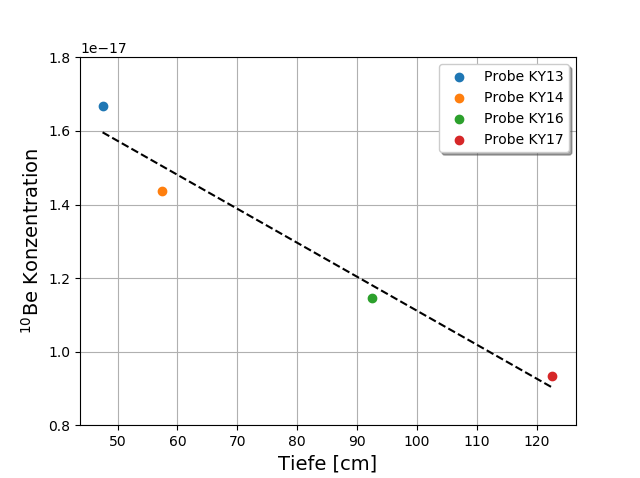
\includegraphics[width=0.7\linewidth]{Pictures/10be_konzentration.png}
  \caption{Berechnete Konzentration von $^9$Be in den Proben in Abhängigkeit von der Tiefe innerhalb der Probe, mit linearen Fit.}
  \label{deep}
\end{figure}
\clearpage

\section{Diskussion}

Alle Aufgabenteile konnten erfolgreich abgeschlossen werden.

Im Niedrigenergiebereich wurden fünf verschiedene Proben auf ihre Zusammensetzung untersucht.
Dabei konnten in der 153BeO die Teilchen $^{16}$O$^{1-}$, $^{9}$Be$^{16}$O$^{1-}$ und $^{12}$C$^{16}$O$^{1-}$ bzw. $^{28}$Si$^{1-}$ nachgewiesen werden.
In den anderen Proben konnten diverse andere Teilchen, darunter bereits erwähnte mit anderen Nukliden sowie AlO gefunden werden.
Zusätzlich wurden einige unbekannte Stoffe gefunden, die wir in diesem Praktikum nicht genauer identifizieren konnten.
Mit einer genauerem Untersuchung der Probe bzw. genaueren Wissen über potentiell vorkommende Elemente sollte das aber auch möglich sein.

Im Hochenergiebereich wurde nur eine Probe untersucht.
Bei dieser wurden die Nuklide $^{9}$Be, $^{10}$Be, $^{12}$C, $^{16}$O und $^{26}$Al in verschiedenen Ladungszuständen gefunden.
Hier ist teilweise eine recht große Ungenauigkeit zwischen berechneter Masse und dem Nuklid vorhanden.
Dies lässt sich zumindest teilweise auf die unbekannten Ungenauigkeiten der Messung zurückführen.
Möglicherweise wurden hier auch einzelne Ionen fehlgedeutet.
Mit Kenntnis der Ursache der Ungenauigkeiten könnte dies genauer werden.

Weiterhin wurde die Detektion und Identifikation von $^{10}\text{Be}$ in einer Gasgefüllten Ionisationsdetektor vorgenommen.
Eine Trennung von den meisten unerwünschten Nukliden die nach dem Beschleuniger auftreten erfolgt durch einen Ablenkmagneten und einen ESA.
Aber auch das Isotop $^{9}\text{Be}$ kann gefunden werden, obwohl man es eigentlich durch Vorselektion aussortieren wollte.
Als Ursache dafür wurde die Molekülbildung von $^{9}\text{Be}^{1}\text{H}^{2+}$ angeführt.
Die Identifikation ist trotz des Auftretens des Isobars $^{10}\text{B}$ möglich.
Es ist sogar möglich das Isobar quantitativ im Spektrum von $^{10}\text{Be}$ zu trennen, womit grundsätzlich eine genaue Bestimmung des Anteils des radioaktiven Isotops $^{10}\text{Be}$ möglich ist, und damit die eigentliche Altersbestimmung.

Die Anteilsbestimmung wurde im letzten Versuchsteil vorgenommen.
Die Konzentration des Radionuklides $^{10}$Be wurde dazu in vier verschiedenen Proben berechnet.
Die Ergebnisse dafür sind in Tab. \ref{dis_con} zu sehen.
\begin{table}[h]
\centering
\caption{Gemessene Werte zur Berechnung der $^{10}$Be Konzentration in den Proben.}
\begin{tabular}{|c |c| c|}
\hline
Probe& $\frac{\text{Atome}}{\si{\gram}}$ & mittlere Tiefe [cm] \\
\hline
KY13 &  $(\num{1.115} \pm \num{0.050}) \cdot 10^{6} $ & 47,5\\
KY14 &  $(\num{9.61} \pm \num{0.44}) \cdot 10^{5} $ & 57,5 \\
KY16 &  $(\num{7.66} \pm \num{0.36}) \cdot 10^{5} $ & 92,5\\
KY17 &  $(\num{6.23} \pm \num{0.33}) \cdot 10^{5} $ & 112,5\\
\hline
\end{tabular}
\label{dis_con}
\end{table}
Wir konnten feststellen, dass die Konzentration scheinbar linear mit zunehmender Tiefe abnimmt.
Dies haben wir so erklärt, dass $^{10}$Be durch Ereignisse mit kosmischer Strahlung entsteht und tieferliegende Proben aufgrund ihres Alters daher weniger $^{10}$Be enthalten müssen.
Nach dieser Erklärung sollte eigentlich ein exponentieller Abfall stattfinden, was wir aber weder ausschließen noch bestätigen können.
Weitere Proben zur Messung könnten diese Frage aber beantworten.
Eine Verfälschung der Proben durch hochenergetische Strahlung aus anderen Quellen ist potentiell möglich, würde aber nichts am Abnehmen der Konzentration ändern.
Eine Neutronenquelle im Inneren der Probe würde das Ergebnis entsprechend ändern können, ist aber unwahrscheinlich.


\nocite{*} % alle resourcen auflisten
\printbibliography

\appendix
\section{Spezieszuordnung}
\label{Appendix_Normen}
Mithilfe einer Norm lassen sich die Permutationen von Ionenspezies bestimmen, die die Peaks im Faraday-Cup am besten beschreiben.
Zuerst wurden die gemessenen Magnetstromstärken-Peaks $\vec{P}_{\text{exp}}$ ermittelt.
Aus diesen wurden die Verhältnisse $\vec{r}_{\text{exp}}$ gebildet.
Dann wurde für die möglichen Ionenspezies $\vec{P}_{\text{möglich}}$ in der Probe das Verhältnis $\frac{\sqrt{m_{\text{ion, möglich}}}}{q_{\text{ion, möglich}}}$ gebildet.
Die Ionenspezies wurden nach diesem Verhältnis geordnet und die erwähnten, geordneten Permutationen $\vec{\nu}(k)$ gebildet.
(Nur Permutationen in dem die Reihenfolge der Elemente nicht vertauscht wird, aber Elemente weggelassen werden können.)
Für diese Permutationen wurde dann ebenfalls das Verhältnis $\vec{r}_{\text{möglich}\ \nu_{i}(k)}$, diesmal von $\frac{\sqrt{m_{\text{ion, möglich}}}}{q_{\text{ion, möglich}}}$, erstellt.
(Das ist ein Vektor für jede Permutation.)
Dann wurde mithilfe der euklidischen Norm der \glqq Abstand\grqq{} der Verhältnisse gebildet:
\begin{gather}
    \norm{\vec{r}_{\text{exp}}-\vec{r}_{\text{möglich}\ \nu_{i}(k)}} = \sqrt{\sum_{n}(\vec{r}_{\text{exp}\ n}-\vec{r}_{\text{möglich}\ \nu_{i}(k),n})^{2}}
\end{gather}
(In Anlehnung an die Methode der kleinsten Fehlerquadrate. Man könnte die Wurzel auch weglassen. Da die Wurzelfunktion monoton ist ändert sie die Reihenfolge später nicht.)
Die Permutation mit der kleinsten Norm ist dann gerade die beste Zuordnung der Ionenspezies zu den Peaks.


% ----- DOKUMENT ENDE -----

\end{document}
